%------------------------------------------------------------------------------%
% Esse arquivo é um exemplo do uso da classe profmat-cefet
% ele contem algumas informações sobre como instalar o LaTeX e a classe
% e como usá-los para escrever sua dissertação.
%
% A classe foi desenvolvida para fornecer uma formatação uniforme e 
% remover do aluno a responsabilidade por escrever segundo os padrões 
% exigidos pelo Profmat no Cefet-MG
%
% Esta classe é baseada na classe book do LaTeX
%
% Estas opções são herdadas da classe base
%    - draft   - Produz uma versão de rascunho do documento final
%    - fleqn   - Alinha as equações a esquerda
%
% Esta classe oferece mais uma opção para definir a formatação geral do texto
%    - short   - Remove a maior parte do preambulo, essa opção deve ser usada
%                nas versões preliminares do texto, sendo removida na versão 
%                final.
%
% Criado por Luis Alberto D'Afonseca
% luis.dafonseca@gmail.com
%------------------------------------------------------------------------------%
\documentclass[fleqn]{profmat-cefet}

% A seguir são incluídos alguns pacotes opcionais que podem ser uteis para 
% a formatação da sua dissertação. Você pode remove-los se não for usá-los.

% Este pacote permite dividir a página em várias colunas
% Veja um exemplo na Lista de Símbolos
\usepackage{multicol}

% Este pacote controla os ambientes de listas
% Veja um exemplo na Lista de Símbolos
\usepackage{enumitem}

% Este pacote permite incluir figuras rodeadas de texto
% Veja exemplos na Introdução
\usepackage{wrapfig}

% Este pacote permite a criação de sub figuras
% Veja um exemplo nas Miscelâneas
\usepackage[format=hang,labelfont=normalfont]{subcaption}

% Esse pacote é usado para criar tabelas que serão dividas em mais do que 
% uma página. Veja um exemplo na seção subsec:classe_e_pacotes_usados
\usepackage{longtable}

% Esse pacote permite escrever frações de forma compacta, veja um exemplo
% no Capítulo 5
\usepackage{xfrac}

% Exemplo da criação de comandos
%------------------------------------------------------------------------------%

% Criando comandos para simplificar a digitação e padronizar a formatação 
\newcommand{\BibTeX}   {\textsc{Bib}\TeX}
\newcommand{\MiKTeX}   {\textsc{MiK}\TeX}
\newcommand{\TeXstudio}{\TeX\textsf{studio}}
\newcommand{\JabRef}   {\textsf{JabRef}}
\newcommand{\texfile}  {\texttt{dissertacao.tex}}
\newcommand{\bibfile}  {\texttt{dissertacao.bib}}
\newcommand{\texdir}   {\texttt{dissertacao}}

% Esse comando declara uma nova função para ser usada no modo matemático
\DeclareMathOperator{\angulo}{\hat{a}ngulo}

% Informações sobre a dissertação
% Substitua pelas informações referentes a sua dissertação
%------------------------------------------------------------------------------%

% Informe seu nome
% Se seu sobrenome for composto use o til (~) como espaço não separável
\autor{Sidney Otavio Oliveira Do Nascimento}

% Informe o título da sua dissertação
\title{Como Produzir um tcc Dentro Das Normas Da UFAL}

% Informe a data da defesa no formato {DD}{MM}{AAAA}
\date{18}{11}{2021}

% Informe os nomes dos membros da banca
% Você pode fornecer entre 3 e 6 nomes nessa lista
% Coloque apenas os nomes de cada professor, não inclua títulos.
%
% ATENÇÃO: O caractere % no final de cada linha é necessário!
%
\banca
{
  Tales de Mileto      \\
  Ada Lovela           \\
  Carl Friedrich Gauss
}

% Informe o orientador e coorientadores
\orientador{Carl Friedrich Gauss}
\coorientacao{Ada Lovelace}

%------------------------------------------------------------------------------%
\begin{document}

% Dedicatória e agradecimentos são opcionais.
% Caso queira você pode simplesmente remover esses campos, 
% mas não mude a ordem deles

%------------------------------------------------------------------------------%
\begin{dedication} 

% Escreva aqui sua dedicatória
Dedico esse trabalho aos Números Irracionais!

\end{dedication}

%------------------------------------------------------------------------------%
\begin{acknowledgement} 

% Escreva aqui os agradecimentos

\noindent
Agradeço as nove musas inspiradoras Calíope, Clio, Erato, Euterpe, Melpômene,
Polímnia, Tália, Terpsícore, Urânia.

%
% O agradecimento abaixo é exigido pela CAPES para todas as dissertações
%
\vspace{2\baselineskip}\noindent
O presente trabalho foi realizado com apoio da Coordenação de Aperfeiçoamento 
de Pessoal de Nível Superior -- Brasil (CAPES) -- Código de Financiamento 001.

\end{acknowledgement}

% Resumo e Abstract
% O resumo e o abstract são mandatórios e devem permanecer nessa posição
%------------------------------------------------------------------------------%
\begin{Resumo}

% Substitua o texto aleatório pelo resumo da sua dissertação.

Esse texto é um exemplo do uso da classe criada para formatar
a dissertação de Mestrado para o PROFMAT no CEFET-MG com o uso do \LaTeX{}.
O Capítulo~\ref{cap:introducao} contem uma apresentação 
da classe, como ela deve ser usada e os comandos criados por 
ela. Além desse texto recomendo também ler com cuidado os comentários escritos
dento do arquivo \texfile{}, eles trazem algumas regras e 
sugestões sobre como preencher algumas partes do texto.
Grande parte do texto é gerado aleatoriamente apenas para preencher as páginas. 
Entretanto, dentro desse texto aleatório existem muitas equações matemáticas, 
figuras e tabelas que podem ser usadas como exemplos caso deseja incluir
algo semelhante em sua dissertação.

\PalavrasChave Matemática. Ensino. Ciência.

\end{Resumo}

%------------------------------------------------------------------------------%
\begin{Abstract}

% Substitua o texto aleatório pelo abstract da sua dissertação.

Offices parties lasting outward nothing age few resolve. Impression to
discretion understood to we interested he excellence. Him remarkably use
projection collecting. Going about eat forty world has round miles. Attention
affection at my preferred offending shameless me if agreeable. Life lain held
calm and true neat she. Much feet each so went no from. Truth began maids linen
an mr to after. 
It allowance prevailed enjoyment in it. Calling observe for who pressed raising
his. Can connection instrument astonished unaffected his motionless preference.
Announcing say boy precaution unaffected difficulty alteration him. Above be
would at so going heard. Engaged at village at am equally proceed. Settle nay
length almost ham direct extent. Agreement for listening remainder get attention
law acuteness day. Now whatever surprise resolved elegance indulged own way
outlived. 

\Keywords Mathematics. Teaching. Science.

\end{Abstract}

% A lista de símbolos é opcional, mantenha-a apenas se for necessária
%------------------------------------------------------------------------------%
\chapter*{Lista de Símbolos}

\noindent
Símbolos e notações utilizadas neste trabalho:

\begin{multicols}{2}
    
    \begin{description}[labelsep=1em]
        \item[$\alpha$]   Letra grega Alfa
        \item[$\beta$]    Letra grega Beta
        \item[$\gamma$]   Letra grega Gama
        \item[$\delta$]   Letra grega Delta
        \item[$\epsilon$] Letra grega Épsilon
        \item[$\zeta$]    Letra grega Zeta
        \item[$\eta$]     Letra grega Eta
        \item[$\theta$]   Letra grega Teta
        \item[$\iota$]    Letra grega Iota
        \item[$\kappa$]   Letra grega Kapa
        \item[$\lambda$]  Letra grega Lambda
        \item[$\mu$]      Letra grega Mi
        \item[$\nu$]      Letra grega Ni
        \item[$\xi$]      Letra grega Xi
        \item[$o$]        Letra grega Ômicron
        \item[$\pi$]      Letra grega Pi
        \item[$\rho$]     Letra grega Rô
        \item[$\sigma$]   Letra grega Sigma
        \item[$\tau$]     Letra grega Tau
        \item[$\upsilon$] Letra grega Upsilon
        \item[$\phi$]     Letra grega Fi
        \item[$\chi$]     Letra grega Chi
        \item[$\psi$]     Letra grega Psi
        \item[$\omega$]   Letra grega Ômega
    \end{description}
    
\end{multicols}


% A lista de abreviaturas é opcional, inclua-a se necessário
%------------------------------------------------------------------------------%

%% \chapter*{Lista de Abreviaturas}

%------------------------------------------------------------------------------%

% A lista de figuras é opcional remova se desejar
\listoffigures

% A lista de tabelas é opcional remova se desejar
\listoftables

% O sumário é mandatório
\tableofcontents

%------------------------------------------------------------------------------%
%------------------------------------------------------------------------------%
%------------------------------------------------------------------------------%
\chapter{Introdução}
\label{cap:introducao}

Nesse texto apresentamos apenas as técnicas necessárias para usar
apropriadamente a classe \LaTeX{} criada para formatar 
a dissertação do PROFMAT.
Não abordamos aspectos como estilo, conteúdo, vocabulário e formalização 
apropriados para uma dissertação em Matemática. Uma boa referência que 
aborda esses aspectos é o livro ``Manual de Redação Matemática'' publicado
pela SBM \cite{MORAISFILHO:MAN_REDACAO_MAT}.

\begin{figure}
    \centering
    \caption{Primeiros passos no \LaTeX.}
    \label{fig:starting_latex}
    
\includegraphics[width=0.4\linewidth]{figs/latex-pet}
    \\ Fonte: Lamport 1985 \cite{LAMPORT:LATEX}
\end{figure}

Essa classe foi criada para facilitar a digitação em \LaTeX{} 
de dissertações de mestrado do PROFMAT.
Essa classe define todas as formatações de texto, papel, bibliografia e outras,
seguindo as normas do CEFET-MG. 
Ela também produz, automaticamente, as páginas do preâmbulo do trabalho, tais 
como capa, declaração, folha de assinaturas e similares. Dessa forma, 
o aluno não precisa empenhar seu tempo para seguir esses padrões podendo 
se dedicar a produção do conteúdo do trabalho.

O arquivo \texfile{} é um exemplo do uso da classe. Você pode
compilá-lo e ver como a classe formata a dissertação. Ele também inclui vários
exemplos de equações, tabelas e figuras em \LaTeX{} que podem ser uteis
quando o aluno desejar obter algum resultado específico.

Este texto descreve o uso da classe e suas opções, porém, assume que o
leitor saiba como usar o \LaTeX{}. Caso o aluno precise de ajuda com o \LaTeX{}
ele pode utilizar uma das várias apostilas e páginas de \emph{internet} disponíveis.
Alguns exemplos são as apostilas
\begin{itemize}
    \item ``Introdução ao \LaTeX{}'' do Prof. Reginaldo da UFMG \cite{REGINALDO:LATEX}
    \item ``Minicurso de \LaTeX{}'' utilizada por Raniere Silva no IMECC--UNICAMP \cite{RANIERE:LATEX}
    \item ``Curso de Introdução ao \LaTeX{}'' do Prof. Márcio da Universidade Estadual Vale do Acaraú \cite{MARCIO:LATEX}
\end{itemize}

Caso você ainda não tenha o \LaTeX{} instalado no seu computador, veja a
Seção~\ref{sec:como_instalar_o_latex}, 
se você já tem o \LaTeX{} e a classe instalados pode pular direto para a
Seção~\ref{sec:como_usar_essa_classe}.

Como essa classe não é uma classe padrão
distribuída juntamente com o \LaTeX{}, você vai precisar copiar os arquivos da
classe na pasta do seu trabalho. Esse procedimento está descrito na
Seção~\ref{sec:como_usar_essa_classe}.

Se você já tem o \LaTeX{} e a classe instalados pode pular direto para a
Seção~\ref{sec:como_usar_essa_classe}.

Uma das tarefas que oferecem mais dificuldade para quem está iniciado no uso do
\LaTeX{} é a construção do banco de dados para a bibliografia.  Por isso, o
Capítulo~\ref{cap:como_escrever_a_bibliografia} traz instruções mais detalhadas
de como isso pode ser feito com o auxilio do \BibTeX{}.

\begin{figure}
	\centering
	\caption{Captura de tela do Editor de Equações Online}
	\label{fig:editor-equacoes}
	\fbox{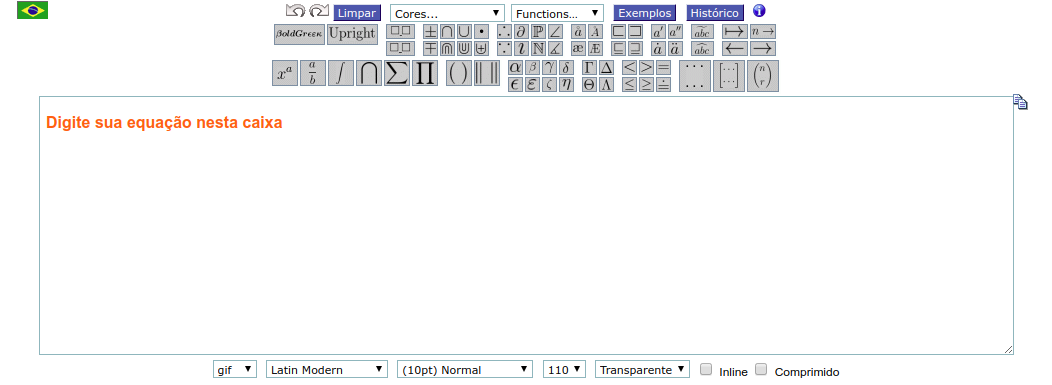
\includegraphics[width=0.7\linewidth]{figs/editor-equacoes}}
	\\ Fonte \url{www.codecogs.com}
\end{figure}

O Capítulo~\ref{cap:exemplos_de_expressoes_matematicas} apresenta várias 
formulas matemáticas que podem ser usadas como exemplos. Veja se alguma
expressão desse capítulo é semelhante ao que deseja produzir e 
adapte o código para as suas necessidades. Quem desejar
usar uma ferramenta gráfica para gerar as expressões em \LaTeX{}
pode usar a página 
\begin{center}
    \url{https://www.codecogs.com/latex/eqneditor.php?lang=pt-br}
\end{center}
que oferece a possibilidade de escrever as expressões selecionando os 
símbolos de um menu, como mostra a Figura~\ref{fig:editor-equacoes}.

O Capítulo~\ref{cap:exemplos_de_tabelas} apresenta vários exemplos de tabelas
e o Capítulo~\ref{cap:exemplos_de_teoremas} ilustra o uso dos diversos
tipos de ambientes de teoremas.
Enquanto que, o Capítulo~\ref{cap:misselaneas_de_exemplos}
exibe exemplos de diversas formas de uso do \LaTeX.

\textbf{Atenção:} Essa classe está preparada para o uso da codificação
\textsf{utf8} e vai produzir resultados espúrios se usada com texto escrito no
formato \textsf{latin1}, que é considerado obsoleto. Para mais informações veja
a Seção~\ref{sec:como_instalar_o_latex}.

%------------------------------------------------------------------------------%
\chapter{Usando o \LaTeX}
\label{cap:como_escrever_uma_dissertacao}

Nesse capítulo descrevemos como instalar o \LaTeX{} e a classe e como usá-los
para escrever sua dissertação.

%------------------------------------------------------------------------------%
\section{Como Instalar o \LaTeX{}}
\label{sec:como_instalar_o_latex}

A seguir está uma lista passo a passo para a instalação do \LaTeX{} no Windows.
Porém, antes da instalação, é importante esclarecer alguns pontos, começando com
um pouquinho de história. O \LaTeX{} foi originalmente escrito por Leslie
Lamport na década de 1980, baseado no \TeX{} que foi escrito por Donald Knuth e
distribuído em 1978. A primeira versão do Microsoft Windows a ser amplamente
distribuída foi a Windows 3.1 lançada em 1992. Esse ponto é importante para
esclarecer porque o \LaTeX{} é diferente da maioria dos programas Windows,
simplesmente ele é muito anterior a definição dos padrões que os programa
Windows seguem. Além disso, um dos principais objetivos do \LaTeX{} é a
consistência, ou seja, o mesmo código deve sempre gerar o mesmo resultado, por
isso suas atualizações evitam fazer grandes alterações.

Uma consequência desta história é que \LaTeX{} não possui interface gráfica,
elas só seriam popularizadas mais de uma década depois de sua criação. Dessa
forma para usarmos o \LaTeX{} no Windows precisamos instalar dois pacotes
\begin{itemize}
    \item \MiKTeX{} que fornece o \LaTeX{} propriamente dito e outros 
    programas auxiliares
    \item e uma interface gráfica para usá-lo.
\end{itemize} 
Existem diversas interfaces gráficas para o \LaTeX{} disponíveis, cada um pode
usar a que preferir, essa escolha não influencia no resultado gerado.  O único
cuidado é escolher uma interface que realmente use o \LaTeX{} e não alguma das
suas variações.

Caso alguém tenha curiosidade, essa página tem uma lista de editores \LaTeX{}
\begin{center}
    \url{https://en.wikipedia.org/wiki/Comparison\_of\_TeX\_editors}
\end{center}
Qualquer editor que edite o código (source) e tenha suporte para unicode
(\textsf{utf8}) pode ser usado. Recomendo o \TeXstudio{} pois é gratuito e tem
disponíveis as funcionalidades mais importantes.

Outra consequência do \LaTeX{} ser um programa desenvolvido das décadas de 70 e
80 é que ele originalmente só reconhecia os caracteres \textsf{ASC-II}, ou seja,
letras sem acentuação, números e poucos outros símbolos. Nada de acentos,
cedilhas, letras gregas ou qualquer outra invencionice. Originalmente era
necessário digitar um comando para incluir cada acento, por exemplo, para
escrever ``ação'' era necessário digitar \lstinline!a\c{c}\~ao!. Para resolver
esse problema foi criado um pacote chamado \textsf{inputenc}, que permite a
digitação de caracteres especiais dentro do arquivo \textsf{tex}, porém, ao
longo da história, várias codificações diferentes foram criadas. O padrão atual
é o \textsf{utf8}, por isso devemos usar o \textsf{inputenc} com essa
codificação.

Entretanto, há algum tempo atrás, os computadores Windows utilizavam outras
codificações, entre elas a usada para o português era a \textsf{latin1}. Por
isso, alguns arquivos \textsf{tex}, ainda circulando hoje em dia, usam essa
codificação. 

\subsection{Instalando o \textsf{MiKTeX}}

É possível que a página do \MiKTeX{} apresente alguma alteração entre o momento
em que esse texto foi escrito e o momento em que você estiver fazendo a
instalação. No momento em que esse texto foi escrito a versão mais atualizada do
\MiKTeX{} era a versão \miktexversion{}. Instale a ultima versão disponível no
momento em que estiver realizando a instalação.  Em caso de dúvidas entre em
contato.

{\color{red}\textbf{ATENÇÃO}}: Instale a versão \textbf{completa} do \MiKTeX{} e
não a versão \textbf{básica}, isso é, {\color{red}\textbf{não}} baixe o arquivo
\texttt{basic-miktex-\miktexversion-x64.exe}.

\begin{enumerate}
    \item Download do instalador
    \begin{enumerate}
        \item Entre na página do \MiKTeX{}: \url{http://miktex.org/download}
        \item {\color{red}\textbf{NÃO}} clique no botão de download!
        \item Selecione a aba \textsf{All Downloads}.
        \item Selecione a opção \textbf{Net Installer}, escolha 32 ou 64 bits de acordo com seu computador
        \item Dependendo do seu computador, baixe o arquivo \texttt{setup-\miktexversion-x64.exe}
                 ou o arquivo \texttt{setup-\miktexversion-x32.exe}
    \end{enumerate}
    \item Baixando o \LaTeX{}
    \begin{enumerate}
        \item Execute o instalador \textsf{setup-\miktexversion{}}.
        \item Permita que o programa faça alterações no seu computador.
        \item Aceite as condições de uso.
        \item Selecione \textsf{Download MiKTeX} e Avance.
        \item Selecione \textsf{Complete MiKTeX} e Avance.
        \item Escolha de qual repositório fazer o download. Escolha qualquer endereço no Brasil.
        \item Escolha onde salvar o download, pode ser no endereço sugerido pelo programa e Avance.
        \item Confirme o download clicando \textsf{start}.
        \item Aguarde o download. Vai demorar um pouco, pois você está baixando o \LaTeX{} com todos seus pacotes.
        \item Quando o download terminar, finalize o programa clicando em avançar .
    \end{enumerate}
    \item Instalação do \LaTeX{}
    \begin{enumerate}
        \item Execute novamente o programa \textsf{setup-\miktexversion{}}.
        \item Aceite novamente os termos de uso.
        \item Selecione \textsf{Install MiKTeX}.  Essa opção já deve estar selecionada por padrão.
        \item Selecione \textsf{Complete MiKTeX}. Essa opção já deve estar selecionada por padrão.
        \item Selecione \textsf{Anyone who uses this computer}. \\
        Assim todos os usuários do computador podem usar o \LaTeX{}.
        \item Selecione de onde o \LaTeX{} será instalado, isto é, a pasta onde o download foi feito. \\
        O programa já deve oferecer a opção correta como padrão.
        \item Selecione onde o \LaTeX{} será instalado. \\
        Recomendo manter a pasta sugerida pelo programa.
        \item Selecione o formato do papel e como os pacotes faltantes devem ser instalados. \\
        Recomendo manter os padrões A4 e \textsf{Ask me first}.
        \item Confirme a instalação.
        \item Aguarde a instalação, ela vai levar algum tempo, então, tenha paciência!
    \end{enumerate}
\end{enumerate}

\subsection{Instalando o \TeXstudio{}}

\begin{enumerate}
    \item Entre na página do \TeXstudio{}: \url{http://www.texstudio.org}
    \item No meno a esquerda, clique em Download 
    \item Baixe o programa, clicando no link download associado a versão adequada para seu Windows
    \item Execute o programa baixado: \textsf{texstudio-2.12.10-win-qt5.exe}
    \item Autorize o programa a fazer alterações no seu computador
    \item Selecione a Linguagem \textsf{Português (Brasil)}
    \item Selecione o local de destino, recomendo deixar opção padrão
    \item Selecione a pasta no menu,    recomendo deixar opção padrão
    \item Aceite que as extensões \textsf{.tex} e \textsf{.txss} sejam associadas ao \TeXstudio{}
    \item Confirme a instalação
\end{enumerate}

\subsection{Testando o \LaTeX{}}

\begin{enumerate}
    \item Rode o \TeXstudio{}
    \item Abra o arquivo \texfile{} distribuído junto com a Classe
    \item Clique no botão verde igual ao botão de avanço rápido 
        
\includegraphics[height=0.7\baselineskip]{figs/fast-forward}
    \item Ele deve compilar sem erros e exibir um \textsf{pdf} que deve se parecer com uma dissertação de mestrado
    \item Verifique se a bibliografia aparece no final da dissertação. Caso não apareça siga os seguintes passos
    \begin{enumerate}
        \item No menu, selecione a opção: \texttt{Tools-Bibliography}
        \item Recompile o texto clicando no botão 
            
\includegraphics[height=0.7\baselineskip]{figs/fast-forward}
    \end{enumerate}
\end{enumerate}

%------------------------------------------------------------------------------%
\section{Como Usar Essa Classe}
\label{sec:como_usar_essa_classe}

A função dela é facilitar a formatação de dissertações para o Mestrado Profmat,
assim ela inclui automaticamente vários pacotes comumente usados, por exemplo,
para a digitação de textos em português, símbolos matemáticos e inclusão de
figuras. A lista completa dos pacotes usados está na
Seção~\ref{sec:classe_e_pacotes_usados}. Porém, sua função mais importante 
é formatar o texto nos moldes exigidos pela universidade. 

Essa classe é usada da mesma forma que as classes predefinidas no 
\LaTeX{}: \lstinline!article!, \lstinline!report!, \lstinline!book!. 
Porém, como não é distribuída junto com o \LaTeX{} é necessário que o arquivo
que a define esteja sempre na mesma pasta que o arquivo que contem o texto em
\LaTeX{}, por exemplo, o arquivo \texfile{}.

Para usar a classe a forma mais simples é copiar toda a pasta que foi
distribuída para uma nova pasta, chamada de \texdir{}, por exemplo.
Nessa nova pasta abra o arquivo \texfile{} e substitua o texto
original pelo texto da sua dissertação.

De modo geral a classe é usada como qualquer outra classe \LaTeX, 
basta especificá-la no comando
\textsf{\mbox{documentclass}}, no início do arquivo \textsf{tex}.
\begin{lstlisting}
\documentclass[(*\textit{opções}*)]{(*\getclass*)}
\end{lstlisting}

Como as demais classes, essa aceita algumas opções listadas na tabela a seguir. 
As opções \lstinline!draft! e \lstinline!fleqn! são herdadas da classe base
\lstinline!book!. \lstinline!short! remove as páginas iniciais da
dissertação sendo usada durante a escrita da dissertação e removida na versão
final que vai ser enviada a banca.
\begin{center}
    \vspace{0.5\baselineskip}
    \begin{tabular}{p{2cm}p{11cm}}                                                           \hline
        Opção                 & Efeito                                                       \\ \hline
        {\lstinline!draft!}   & Compila uma versão de rascunho (não inclui as figuras)       \\
        {\lstinline!fleqn!}   & Alinha as equações a esquerda                                \\
        {\lstinline!short!}   & Remove as páginas do preambulo como declaração e assinaturas \\ \hline
    \end{tabular}
    \vspace{0.5\baselineskip}
\end{center}

%------------------------------------------------------------------------------%
\section{Autor, Orientador, Título e Banca}
\label{sec:autor_orientador_titulo_e_banca}

Como em outras classes, o nome do autor, título da dissertação e outras
informações devem ser passadas por comandos e a classe cria a capa utilizando
essa informação.

Como o português possui declinações baseadas em gênero (o/a) os comandos que
definem o autor e o orientador dessa classe existem em duas versões, uma
para o gênero masculino e outra para o gênero feminino.
\begin{center}
    \vspace{0.5\baselineskip}
    \begin{tabular}{ll}
    	\hline
    	Comando                           & Função                                                         \\ \hline
    	{\lstinline!\autor!}              & Define o nome do autor da dissertação                          \\
    	{\lstinline!\autora!}             & O mesmo que {\lstinline!\autor!} para o gênero feminino        \\
    	{\lstinline!\orientador!}         & Define o nome do orientador da dissertação                     \\
    	{\lstinline!\orientadora!}        & O mesmo que {\lstinline!\orientador!} para o gênero feminino   \\
    	{\lstinline!\coorientador!}       & Define o nome do coorientador da dissertação                   \\
    	{\lstinline!\coorientadora!}      & O mesmo que {\lstinline!\coorientador!} para o gênero feminino \\
    	{\lstinline!\coorientadores!}     & Usado no caso de dois coorientadores                           \\
    	{\lstinline!\coorientadoras!}     & Usado no caso de duas coorientadoras                           \\
    	{\lstinline!\title!}              & Define o título da dissertação                                 \\
    	{\lstinline!\date{DD}{MM}{AAAA}!} & Define data da defesa no formato dia, mês e ano                \\
    	{\lstinline!\board!}              & Lista os nomes dos membros da banca                            \\ \hline
    \end{tabular}
    \vspace{0.5\baselineskip}
\end{center}

Os comandos para definir autor(a), orientador(a) e coorientador(a) devem ser
usados apenas uma vez no gênero masculino ou feminino, singular ou plural.
Dependendo do modelo da dissertação algumas dessas informações podem não ser
utilizadas ou mesmo necessárias.

Uma atenção especial deve ser dada a determinação dos membros da banca pelo
comando \lstinline!\board!. É possível listar entre 3 e 6 membros para a banca,
os nomes vão aparecer na página de assinaturas na ordem em que forem listados.
Como esse comando tem um número variável de parâmetros, ele interrompe a leitura
dos parâmetros assim que encontra um espaço em branco ou fim de linha, o que
pode causar confusão a alguns usuários. Uma solução é colocar o símbolo de
comentário \lstinline{%}
logo após cada parâmetro do comando, como no exemplo a seguir.
    
\begin{lstlisting}
% Informe seu nome
\autor{(*Luis Albero D'Afonseca*)}

% (*\color{commentcolor} Informe o título da sua dissertação*)
\title  {(*Estudo Matemático da Teoria Abstrata*)}

% (*\color{commentcolor} Informe a data da defesa no formato *){DD}{MM}{AAAA}
\date{31}{02}{2016}

% (*\color{commentcolor} Informe os nomes dos membros da banca*)
% (*\color{commentcolor} Você pode fornecer entre 3 e 6 nomes nessa lista*)
% (*\color{commentcolor} ATENÇÃO: O caractere*) % (*\color{commentcolor} no final das linhas é necessário!*)
\board{(*Tales de Mileto*)}%
      {(*Leonhard Euler*)}%
      {(*Ada Lovelace*)\\(*(Coorientadora)*)}%
      {(*Carl Friedrich Gauss*)\\(*(Orientador)*)}

% (*\color{commentcolor} Informe o orientador e coorientador caso exista*)
\orientador{(*Carl Friedrich Gauss*)}
\coorientadora{(*Ada Lovelace*)}
\end{lstlisting}

%------------------------------------------------------------------------------%
\section{Novos Ambientes}
\label{sec:novos_ambientes}

No preambulo das dissertações é comum que o aluno dedique sua dissertação e faça
agradecimentos. Para esse fim, essa classe cria os ambientes 
\lstinline!dedication!, 
\lstinline!acknowledgement! e
\lstinline!biography!.
Basta criar os ambientes e digitar o texto desejado em seu interior,
como no exemplo
\begin{lstlisting}
\begin{dedication} 
    (*Dedico esse trabalho aos números irracionais!*)
\end{dedication}

\begin{acknowledgement} 
  (*Agradeço*) as nove musas inspiradoras (*Calíope*), Clio, Erato, 
  Euterpe, (*Melpômene*), (*Polímnia*), (*Tália*), (*Terpsícore*), (*Urânia.*)
\end{acknowledgement}

\begin{biography} 
    (*Eu sou o máximo!*)
\end{biography}
\end{lstlisting}

Também estão disponíveis ambientes para o resumo e para o abstract, 
veja exemplos no arquivo \texfile{}.

%------------------------------------------------------------------------------%
\section{Novos Comandos}
\label{sec:novos_comandos}

Para agilizar o processo de digitação da dissertação e para padronizar os
formatos, a classe cria os seguintes ambientes para teoremas
(\lstinline!newtheorem!):
\begin{center}
    \begin{tabular}{lll}
            \hline
            Ambiente               & Teorema    & Numeração \\ \hline
            \lstinline!axioma!     & Axioma     & Capítulo  \\
            \lstinline!definicao!  & Definição  & Capítulo  \\
            \lstinline!postulado!  & Postulado  & Capítulo  \\
            \lstinline!proposicao! & Proposição & Capítulo  \\
            \lstinline!lema!       & Lema       & Capítulo  \\
            \lstinline!teorema!    & Teorema    & Capítulo  \\
            \lstinline!corolario!  & Corolário  & Capítulo  \\
            \lstinline!exemplo!    & Exemplo    & Seção     \\
            \lstinline!exercicio!  & Exercício  & Seção     \\ \hline
    \end{tabular}
\end{center}

O nome de algumas funções trigonométricas foram adaptadas
\begin{center}
    \begin{tabular}{llcll}
    	\hline
    	Comando            & Símbolo  & \null\hspace{2cm}\null & Comando               & Símbolo     \\ \hline
    	\lstinline!\sin x! & $\sin x$ &                        & \lstinline!\arcsin x! & $\arcsin x$ \\
    	\lstinline!\tan x! & $\tan x$ &                        & \lstinline!\arctan x! & $\arctan x$ \\
    	\lstinline!\csc x! & $\csc x$ &                        & \lstinline!\arccsc x! & $\arccsc x$ \\
    	\lstinline!\cot x! & $\cot x$ &                        & \lstinline!\arccot x! & $\arccot x$ \\
    	                   &          &                        & \lstinline!\arcsec x! & $\arcsec x$ \\ \hline
    \end{tabular}
\end{center}

Comandos para os conjuntos numéricos mais utilizados
\begin{center}
    \begin{tabular}{lcc}
            \hline
            Conjunto  &    Comando     & Símbolo \\ \hline
            Naturais  & \lstinline!\N! &  $\N$   \\
            Inteiros  & \lstinline!\Z! &  $\Z$   \\
            Racionais & \lstinline!\Q! &  $\Q$   \\
            Reais     & \lstinline!\R! &  $\R$   \\
            Complexos & \lstinline!\C! &  $\C$   \\ \hline
    \end{tabular}
\end{center}

%------------------------------------------------------------------------------%
\section{Páginas de Assinaturas e Ficha Catalográfica}
\label{sec:paginas_de_assinatura_e_ficha_catalografica}

Na versão final da dissertação as páginas de assinaturas e ficha catalográfica
precisam de tratamento especial. A página de assinaturas deve ser
substituída pela folha assinada pelos membros da banca e a ficha catalográfica
é construída em conjunto com a equipe da biblioteca.
Para lidar com esses casos a classe substitui essas páginas com o 
conteúdo de arquivos \textsf{pdf} quando fornecidos.

Por exemplo, para gerar a página de assinaturas o aluno pode imprimir apenas 
essa página do arquivo \textsf{pdf} da sua dissertação e colher as assinaturas 
dos membros da banca. Em seguida, escaneia a folha assinada e salva com o nome
\textsf{assinaturas.pdf}. Agora, basta colocar esse arquivo dentro da pasta 
da dissertação e recompilar o \LaTeX{}. O novo aquivo \textsf{pdf} gerado 
vai conter a folha assinada no local da original sem assinaturas.

Um procedimento semelhante é feito para incluir a ficha catalográfica.
Depois de criada a ficha, salve-a em um arquivo com o nome
\textsf{ficha\_catalografica.pdf} dentro da pasta da dissertação e recompile o 
\LaTeX{}.

%------------------------------------------------------------------------------%
\section{Comentários, Dicas e Sugestões}
\label{sec:comentarios_dicas_e_sugestoes}

\begin{description}
    \item[Nomes, Títulos e Legenadas]
        Use \lstinline!~! (til) para criar espaço não separável e agrupar 
        sobrenomes compostos 

    \item[Evite Erros Obscuros]
        Não use acentos ou símbolos especiais nos \textsf{labels} da bibliografia,
        de equações, das figuras e similares.

    \item[Evite Anacronismos]
        Para criar um ambiente matemático destacado use \\
        \lstinline!\[ x = \sin \alpha \]! \\
        ou ambientes como o \lstinline!equation!. Jamais use a forma ultrapassada \\
        \lstinline!$$ x = \sin \alpha $$!\\
        Esse link apresenta os argumentos do porque devemos seguir esse padrão
        \begin{center}
            \url{http://tex.stackexchange.com/questions/503/why-is-preferable-to}
        \end{center}

\end{description}

%------------------------------------------------------------------------------%
\section{Classe e Pacotes Usados}
\label{sec:classe_e_pacotes_usados}

A Classe Profmat é baseada na classe padrão \lstinline!book! e herda a maioria 
das suas características. Para formatar adequadamente a dissertação, vários 
pacotes foram inseridos na definição da classe e portanto podem ser usados
dentro da dissertação sem precisar serem incluídos novamente. 
Esses pacotes estão listados na tabela a seguir.

\begin{center}
    \begin{longtable}{ll}
        \hline
        Pacote                  & Função                                                       \\ \hline
        \lstinline!abntex2cite! & Formata a bibliografia segundo as regras da ABNT             \\
        \lstinline!ae!          & Evita problemas com as fontes em arquivos \textsf{pdf}       \\
        \lstinline!amsfonts!    & Mais símbolos matemáticos                                    \\
        \lstinline!amsmath!     & Mais símbolos matemáticos                                    \\
        \lstinline!amssymb!     & Mais símbolos matemáticos                                    \\
        \lstinline!amsthm!      & Mais símbolos matemáticos                                    \\
        \lstinline!array!       & Estende os ambientes \lstinline!array! e \lstinline!tabular! \\
        \lstinline!babel!       & Adapta o \LaTeX para o português                             \\
        \lstinline!caption!     & Controla a formatação das legendas                           \\
        \lstinline!changepage!  & Ajustes nas margens do texto                                 \\
        \lstinline!comment!     & Permite comentar trechos do código                           \\
        \lstinline!csquotes!    & Facilita o uso de aspas                                      \\
        \lstinline!etoolbox!    & Adiciona funcionalidades de programação ao \LaTeX            \\
        \lstinline!fancyhdr!    & Controla a formatação dos cabeçalhos                         \\ 
        \lstinline!fontenc!     & Codificação de fonte                                         \\
        \lstinline!geometry!    & Define a geometria da página                                 \\
        \lstinline!graphicx!    & Inclusão de imagens                                          \\
        \lstinline!hyperref!    & Permite a criação de hiperlinks                              \\
        \lstinline!icomma!      & Ajusta o espaçamento da vírgula quando usada em números      \\
        \lstinline!indentfirst! & Inclui indentação no primeiro parágrafo de cada seção        \\
        \lstinline!inputenc!    & Permite a leitura de caracteres com acentuação               \\
        \lstinline!latexsym!    & Mais símbolos matemáticos                                    \\
        \lstinline!microtype!   & Melhorias na tipografia                                      \\
        \lstinline!nccmath!     & Inclui alguns comandos matemáticos                           \\
        \lstinline!pdfpages!    & Inclusão de arquivos \textsf{pdf}                            \\
        \lstinline!placeins!    & Controla o posicionamento de objetos flutuantes              \\
        \lstinline!setspace!    & Controle do espaçamento entre linhas                         \\
        \lstinline!textpos!     & Posicionamento absoluto de texto                             \\
        \lstinline!tikz!        & Cria gráficos diretamente no \LaTeX                          \\
        \lstinline!titlesec!    & Controla a formatação dos títulos                            \\
        \lstinline!tocbibind!   & Inclui a bibliografia no sumário                             \\
        \lstinline!tocstyle!    & Controla o estilo do sumário                                 \\
        \lstinline!xparse!      & Permite o manejo de opções                                   \\
        \hline
    \end{longtable}
\end{center}

Além dos pacotes incluídos pela classe alguns pacotes foram incluído no arquivo \LaTeX{}
para servirem de exemplo da inclusão de pacotes e também ilustrar algumas funcionalidades
úteis. 
\begin{center}
    \begin{longtable}{ll}
        \hline
        Pacote                 & Função                                                        \\ \hline
        \lstinline!enumitem!   & Controla os ambientes de listas                               \\
        \lstinline!longtable!  & Cria tabelas que podem se estender por mais do que uma página \\
        \lstinline!multicol!   & Permite dividir a página em várias colunas                    \\
        \lstinline!subcaption! & Permite a criação de sub figuras com sua legendas             \\
        \lstinline!wrapfig!    & Permite incluir figuras rodeadas de texto                     \\
        \lstinline!xfrac!      & Escreve frações em forma compacta                             \\ \hline
    \end{longtable}
\end{center}

%------------------------------------------------------------------------------%
\section{Arquivos Gerados pelo \LaTeX{}}
\label{sec:arquivos_gerados_pelo_latex}

Ao compilar um arquivo \textsf{tex} o \LaTeX{} gera vários arquivos auxiliares,
esses arquivos podem ser removidos sem nenhuma perda pois serão regerados na
próxima execução do \LaTeX. Uma lista de extensões de arquivos auxiliares é
\begin{center}
    \begin{tabular}{cccccccc}    \hline
        \textsf{.aux} & \textsf{.bbl} & \textsf{.toc} &
        \textsf{.blg} & \textsf{.lof} & \textsf{.log} & 
        \textsf{.out} \\ \hline
    \end{tabular}
\end{center}

O arquivo com a extensão \textsf{.synctex.gz} é gerado pelo \TeXstudio{}
e armazena configurações deste programa referentes a dissertação. Ele também
pode ser removido sem grandes perdas.

Jamais remova arquivos com as extensões a seguir, a menos que saiba muito bem 
o que está fazendo
\begin{center}
    \begin{tabular}{cccc}    \hline
        \textsf{.tex} & \textsf{.bib} & \textsf{.cls} & \textsf{.sty} \\
        \hline
    \end{tabular}
\end{center}

%------------------------------------------------------------------------------%
%------------------------------------------------------------------------------%
%------------------------------------------------------------------------------%
\chapter{Como Escrever a Bibliografia}
\label{cap:como_escrever_a_bibliografia}

%\newcommand{\addbibentry}[1]{\texttt{\makeatletter{@#1}\makeatother}}

A classe do Profmat no Cefet-MG usa o pacote \textsc{abntex2cite}
que é parte da suíte \textsc{ABsurd Norms for TeX}~\cite{ABNTEX}.
Esse pacote usa o \BibTeX{} 
para gerar a lista de referências da dissertação, de acordo com as normas 
estabelecidas pela ABNT~\cite{NBR6023:2000}.

Entre as vantagens de usar uma ferramenta para a construção 
de um banco de dados de referências é que podemos baixar referências prontas da
internet para livros e artigos específicos ou para bibliografias
completas. Além disso, o \BibTeX{} toma conta automaticamente da ordenação
e formatação das referências. 

Essas referências são geradas a partir de entradas em arquivos \texttt{.bib},
Na distribuição da classe existe um arquivo chamado 
\bibfile{} que contém as referências usadas nesse 
texto e que servem como exemplos de citações. 
Os principais tipos de citações são descritos na 
Seção~\ref{sec:principais_tipos_de_referencias} indicando quais campos
devem ser preenchidos e como preenche-los.

%------------------------------------------------------------------------------%
\section{Citando uma Referência no Texto}
\label{sec:citando_uma_referencia_no_texto}

No decorrer do texto, no arquivo \LaTeX{}, sempre que uma citação for necessária
basta incluir o comando \lstinline!\cite{bibtexkey}! onde \lstinline!bibtexkey! é 
a chave usada para identificar cada referência incluída no arquivo 
\bibfile{}. O \TeXstudio{} oferece automaticamente todas as chaves disponíveis, 
não sendo necessário memorizá-las ou digitá-las todas as vezes.

Observe que apenas as referencias citadas no texto são incluídas na bibliografia,
isso é, não basta incluir a referência no arquivo \bibfile{}
para que ela apareça na bibliografia na dissertação, é necessário citá-la
no texto também. 

Além do \lstinline!\cite! o \textsc{abntex2cite} também fornece esses outros comandos
para referências.
\begin{itemize}
\item Citando diretamente uma referência com o comando \lstinline|\cite|: 
\cite{ARAUJO:ABNTEX2CITE} e \cite{MOREIRA:TOP_TEO_NUM}.
\begin{lstlisting}
\cite{ARAUJO:ABNTEX2CITE} e \cite{MOREIRA:TOP_TEO_NUM}.
\end{lstlisting}

\item Fazendo uma citação na linha com o comando \lstinline|\citeonline|: 
\citeonline{ARAUJO:ABNTEX2CITE} e \citeonline{MOREIRA:TOP_TEO_NUM}.
\begin{lstlisting}
\citeonline{ARAUJO:ABNTEX2CITE} e \citeonline{MOREIRA:TOP_TEO_NUM}.
\end{lstlisting}

\item Citando com o nome do autor com o comando \lstinline|\citeauthor|: 
\citeauthor{ARAUJO:ABNTEX2CITE} e \citeauthor{MOREIRA:TOP_TEO_NUM}.
\begin{lstlisting}
\citeauthor{ARAUJO:ABNTEX2CITE} e \citeauthor{MOREIRA:TOP_TEO_NUM}.
\end{lstlisting}

\item Citando com o nome do autor na linha com o comando \lstinline|\citeauthoronline|: 
\citeauthoronline{ARAUJO:ABNTEX2CITE} e \citeauthoronline{MOREIRA:TOP_TEO_NUM}.
\begin{lstlisting}
\citeauthoronline{ARAUJO:ABNTEX2CITE} e 
\citeauthoronline{MOREIRA:TOP_TEO_NUM}.
\end{lstlisting}

\item Citando o ano com o comando \lstinline|\citeyear|: 
\citeyear{ARAUJO:ABNTEX2CITE} e \citeyear{MOREIRA:TOP_TEO_NUM}.
\begin{lstlisting}
\citeyear{ARAUJO:ABNTEX2CITE} e \citeyear{MOREIRA:TOP_TEO_NUM}.
\end{lstlisting}
\end{itemize}

%------------------------------------------------------------------------------%
\section{Ferramentas para Gerenciar a Bibliografia}
\label{sec:ferramenta_para_gerenciar_a_bibliografia}

O arquivo \bibfile{} pode ser editado manualmente usando o 
\TeXstudio{} ou com o uso de um editor próprio para arquivos de bibliografia.
Se você desejar um editor de bibliografia que eu recomendo é o \JabRef{}.
Além disso, esse programa permite baixar da internet as referências prontas.

Os arquivos com as referências bibliográficas tem uma formatação rígida e
pouco intuitiva, gerando resultados inesperados em muitos casos. Uma forma 
de evitar erros na digitação desses arquivos é usar um programa especifico 
para esse fim. Uma opção é o \JabRef{}~\cite{JABREF} que gerencia as referencias 
de forma simples. Para instalá-lo basta seguir as instruções de sua página 
\begin{center}
    \url{http://www.jabref.org}
\end{center}
Se o programa estiver em inglês após a instalação basta configurá-lo para o 
português, entrando do menu \textsf{Opctions -- Preferences} que abre o 
quadro de dialogo de Preferencias. Nesse quadro selecione a aba \textsf{General}
e dentro dessa aba selecione \textsf{Brazilian Portuguese} na opção \textsf{Language}.
Ao reiniciar o programa ele estará com os menus em português.

Como as normas ABNT são estão em dissonância com os padrões internacionais, 
o pacote \textsc{abntex2cite} cria campos e não reconhecidos pelo automaticamente
pelo \JabRef{}. 
É possível fazer as edições a mão quando os campos não são reconhecidos,
porém, pode ser mais simples ajustar as configurações do \JabRef{} para que
ele siga as especificações necessárias para o \textsc{ABsurd Norms for TeX},
para isso siga os passos descritos na página
\begin{center}
    \url{https://github.com/abntex/abntex2/wiki/JabRef}
\end{center}

%------------------------------------------------------------------------------%
\subsection{Problemas com Conversão para Maiúsculas}

Nas suas entradas que ficam o nos arquivos \texttt{.bib} 
você deve tomar cuidado especial com a formatação dos acentos, 
especialmente no campo \texttt{author} que sempre é convertido para maiúsculas. 
Nesses casos é recomendável utilizar a acentuação original do \LaTeX 
usando comandos e não letras acentuadas, como mostra a tabela
\begin{center}
    \begin{tabular}{clcclcclcclcclccl}
            á & \lstinline!{\'a}!  & & 
            à & \lstinline!{\`a}!  & & 
            â & \lstinline!{\^a}!  & & 
            ã & \lstinline!{\~a}!  & & 
            í & \lstinline!{\'\i}! & & 
            ç & \lstinline!{\c c}!
    \end{tabular}
\end{center}
Você não precisa formatar toda a sua entrada desta maneira, 
apenas aquelas que vão ser convertidas para maiúsculas.

%------------------------------------------------------------------------------%
\section{Principais Tipos de Referências}
\label{sec:principais_tipos_de_referencias}

\newcommand{\citeexample}[1]{
  \begin{flushleft}
    \vspace{-\baselineskip}Entrada produzida na bibliografia
  \end{flushleft}
  \begin{center}
    \begin{small}
    \begin{spacing}{1}
      \fbox{\parbox{0.88\linewidth}{
      \hypersetup{citecolor=black}
      \citetext{#1}
      \hypersetup{citecolor=green}
      \vspace{0.2\baselineskip}}}
    \end{spacing}
    \end{small}
  \end{center}
}

Apresentamos nessa seção alguns exemplos dos principais tipos de referências 
seguindo o padrão \textsc{abntex2cite}. Mais informações e exemplos podem 
ser encontrados na documentação do pacote~\cite{ARAUJO:ABNTEX2CITE}.

%------------------------------------------------------------------------------%
\subsection{Livros}

Alguns exemplos de citações de livros são:
\citeauthor{MOREIRA:TOP_TEO_NUM}, 
\citeauthor{CARVALHO:MAT_DISC}, 
\citeauthor{GIRALDO:REC_COMP_ENS_MAT}, 
\citeauthor{GOMEZ:GEO_ANA}, 
\citeauthor{HEFEZ:ARIT}, 
\citeauthor{HEFEZ:EX_RES_ARIT}, 
\citeauthor{HEFEZ:EX_RES_ALG_LIN}, 
\citeauthor{HEFEZ:INTRO_ALG_LIN}, 
\citeauthor{HEFEZ:POLY_EQ_ALG}, 
\citeauthor{LAMPORT:LATEX}, 
\citeauthor{LIMA:NUM_FUNC_R}, 
\citeauthor{MORAISFILHO:MAN_REDACAO_MAT}, 
\citeauthor{MUNIZNETO:FUND_CALC}, 
\citeauthor{MUNIZNETO:GEO}, 
\citeauthor{PITOMBEIRA:TOP_HIST_MAT}, 
\citeauthor{RABELO:AVA_EDUC}, 
\citeauthor{ROUSSEAU:MAT_ATU_1}, 
\citeauthor{ROUSSEAU:MAT_ATU_2} e 
\citeauthor{WAGNER:T_PROB_ELEM}.

Uma entrada para livro no arquivo de bibliografias é feita como segue.
\begin{lstlisting}
@Book{CARVALHO:MAT_DISC,
  Title     = {Matem{\'a}tica Discreta},
  Author    = {Paulo Cezar Pinto Carvalho and 
               Augusto Cezar de Oliveira Morgado},
  Year      = {2015},
  Edition   = {2},
  ISBN      = {9788583370154},
  Pages     = {192},
  Publisher = {SBM},
  Series    = {Cole{\c{c}{\~a}o Profmat},
  Address   = {Rio de Janeiro}
}
\end{lstlisting}
\citeexample{CARVALHO:MAT_DISC}

Quando o livro possuir subtítulo
\begin{lstlisting}
@Book{RABELO:AVA_EDUC,
  Title     = {Avalia{\c{c}}{\~a}o Educacional},
  Subtitle  = {fundamentos, metodologia e aplica{\c{c}}{\~o}es 
               no contexto brasileiro},
  Author    = {Mauro Luiz Rabelo},
  Year      = {2013},
  Edition   = {1},
  ISBN      = {9788583370062},
  Pages     = {260},
  Publisher = {SBM},
  Series    = {Cole{\c{c}}{\~a}o Profmat},
  Address   = {Rio de Janeiro}
}
\end{lstlisting}
\citeexample{RABELO:AVA_EDUC}

%------------------------------------------------------------------------------%
\subsection{Artigos}

Para artigos a entrada não difere muito dos livros, 
um exemplo de citação de um artigo é \citeauthor{LOPES:CELULAR}.

Note nesse exemplo que as chaves podem ser substituídas por aspas duplas para especificar um campo. 
Note também que as iniciais dos itens da referência podem ser em letras maiúsculas ou minúsculas.
\begin{lstlisting}
@Article{LOPES:CELULAR,
  Title     = {O uso do celular em sala de aula como ferramenta 
               pedag{\'o}gica: benef{\'\i}cios e desafios},
  Author    = {P. A. Lopes and C. C. C. Pimenta},
  Year      = {2017},
  Number    = {1},
  Pages     = {52-66},
  Volume    = {3},
  Address   = {Recife - PE},
  Journal   = {Revista Cadernos de Estudos e Pesquisa na 
               Educa{\c{c}}{\~a}o B{\'a}sica},
  Publisher = {{CAP} {UFPE}}
}
\end{lstlisting}
\citeexample{LOPES:CELULAR}

Um exemplo de artigo publicado em anais ou \textit{proceedings} 
de um congresso é \citeauthor{SOUZA:1994}.

Incluímos uma referência a artigos en anis como segue.
\begin{lstlisting}
@InProceedings{SOUZA:1994,
  Title  = {Influ{\^e}ncia da corre{\c{c}}{\~a}o e do
            preparo do solo sobre algumas propriedades
            qu{\'\i}micas do solo cultivado com bananeiras},
  Author = {L. S. Souza and A. L. Borges and J. O. Rezende},
  BookTitle    = {Anais...},
  Year         = {1994},
  Organization = {Reuni\~ao Brasileira de Fertilidade do Solo
                  e Nutri{\c c}\~ao de Plantas},
  Pages        = {3-4},
  Publisher    = {EMBRAPA, CATSA},
  Address             = {Petrolina},
  Conference-Location = {Petrolina},
  Conference-Number   = {21},
  Conference-Year     = {1994}
}
\end{lstlisting}
\citeexample{SOUZA:1994}

%------------------------------------------------------------------------------%
\subsection{Dissertações de Mestrado ou Doutorado}

Em muitos casos citamos dissertações de mestrado ou doutorado, como nesses casos:
\citeauthor{GEOGEBRA:TESE} e
\citeauthor{SOUZA:Bayesiana}.

Para uma dissertação de mestrado usamos a seguinte entrada
\begin{lstlisting}
@MasterThesis{GEOGEBRA:TESE,
  Title  = {{G}eo{G}ebra: Ein {S}oftwaresystem f{\"u}r 
            dynamische {G}eometrie und {A}lgebra der {E}bene},
  Author = {Markus Hohenwarter},
  Year   = {2002-02},
  Note   = {(In German)},
  Type   = {Mestrado em Matemem{\'a}tica},
  School = {Paris Lodron University, Salzburg, Austria}
}
\end{lstlisting}
\citeexample{GEOGEBRA:TESE}

Para uma tese de doutorado usamos \lstinline|@PhdThesis|
e no campo \lstinline|Type| descrevemos a área da tese 
``Doutorado em Matemática'', por exemplo.
    
%------------------------------------------------------------------------------%
\subsection{Leis e Normas}

Citando a norma ABNT NBR6023 \cite{NBR6023:2000} temos a seguinte estrutura
\begin{lstlisting}
@Manual{NBR6023:2000,
  Title        = {{NBR} 6023},
  Year         = {2000},
  Organization = {Associa{\c c}{\~a}o Brasileira de Normas 
                  T{\'e}cnicas},
  Pages        = {22},
  Subtitle     = {Informa{\c{c}}{\~a}o e documenta{\c{c}}{\~a}o
                  -- Refer{\^e}ncias -- Elabora{\c{c}}{\~a}o},
  Address      = {Rio de Janeiro}
}
\end{lstlisting}
\citeexample{NBR6023:2000}

Enquanto que a LDB \cite{LDB} deve ser descrita como
\begin{lstlisting}
@Manual{LDB,
  Title = {Lei de Diretrizes e Bases da Educa{\c{c}}{\~a}o 
           Nacional n. 9394, de 20 de Dezembro de 1996},
  Year  = {1996},
  Note  = {Estabelece as diretrizes e bases da 
           educa{\c{c}}{\~a}o nacional},
  Organization = {Brasil. Minist\'erio da Educa{\c c}{\~a}o},
  Publisher    = {MEC},
  Address      = {Bras{\'\i}lia}
}
\end{lstlisting}
\citeexample{LDB}

%------------------------------------------------------------------------------%
\subsection{Páginas na Internet}

Mesmo não sendo o melhor tipo fonte para trabalhos acadêmicos, 
em alguns casos precisamos citar páginas da internet. 
Esses são alguns exemplos de citações de páginas:
\citeauthor{WIKI:TEO_FUND_ARIT},
\citeauthor{TEXSTUDIO},
\citeauthor{GEOGEBRA} e
\citeauthor{JABREF}.

O \texttt{anbtex2cite} não possui um tipo específico para páginas da internet,
dessa forma citamos as páginas usando uma entrada do tipo \lstinline|@Misc|.
Quando a página da internet não tem autor definido, usamos a entrada 
\begin{lstlisting}
@Misc{WIKI:TEO_FUND_ARIT,
  Title         = {Teorema fundamental da aritm{\'e}tica},
  Url           = {https://pt.wikipedia.org/wiki/
                   Teorema_fundamental_da_(*aritm{\'e}tica*)},
  Year          = {2017-09-13},
  Organization  = {Wikip\'edia},
  UrlAccessDate = {18 de mar{\c{c}}o de 2018}
}
\end{lstlisting}
\citeexample{WIKI:TEO_FUND_ARIT}

Para uma página da internet com autor temos \cite{ABNTEX,ARAUJO:ABNTEX2CITE}. 
A entrada no arquivo de bibliografia fica como a seguir.
\begin{lstlisting}
@Misc{ABNTEX,
  Title    = {O pacote abntex2cite},
  Author   = {Lauro C{\'e}sar Araujo},
  Url      = {http://www.abntex.net.br/},
  Year     = {2015},
  Subtitle = {t{\'o}picos espec{\'\i}ficos da {ABNT} 
              {NBR} 10520:2002 e o estilo bibliogr{\'a}fico
              alfab{\'e}tico (sistema autor-data)},
  UrlAccessDate = {03 de mar{\c{c}}o de 2020}
}
\end{lstlisting}
\citeexample{ABNTEX}

A citação pode ser a um programa, como o Geogebra \cite{GEOGEBRA}, por exemplo
\begin{lstlisting}
@Misc{GEOGEBRA,
  Title  = {{G}eo{G}ebra},
  Author = {Hohenwarter, M. and Borcherds, M. and Ancsin, G. 
            and Bencze, B. and Blossier, M. and Delobelle, A. 
            and Denizet, C. and {\'E}li{\'a}s, J. and Fekete, {\'A} 
            and G{\'a}l, L. and Konecn{\'y}, Z. and Kov{\'a}cs, Z. 
            and Lizelfelner, S. and Parisse, B. and Sturr, G.},
  Url    = {http://www.geogebra.org},
  Year   = {2017},
  UrlAccessDate = {08 de abril de 2018}
}
\end{lstlisting}
\citeexample{GEOGEBRA}

%------------------------------------------------------------------------------%
\subsection{Manuais}

Também podemos citar manuais:
\citeauthor{REGINALDO:LATEX}, 
\citeauthor{MARCIO:LATEX} e
\citeauthor{RANIERE:LATEX}.
Alguns exemplos de manuais não publicados, disponíveis na \textit{internet}.
Uma boa apostila sobre \LaTeX, \cite{REGINALDO:LATEX}
\begin{lstlisting}
@Manual{REGINALDO:LATEX,
  Title         = {Introdu{\c{c}}{\~a}o ao {LaTeX}},
  Author        = {Reginaldo J. Santos},
  Year          = {10-2002},
  Url           = {http://www.mat.ufmg.br/~regi/topicos/intlat.pdf},
  Address       = {Belo Horizonte - MG},
  UrlAccessDate = {18 de mar{\c{c}}o de 2018}
}
\end{lstlisting}
\citeexample{REGINALDO:LATEX}

%------------------------------------------------------------------------------%
\section{Lista de Entradas no \BibTeX}

A tabela a seguir lista as entradas possíveis para o \BibTeX e quais campos são
obrigatórios e opcionais para cada entrada.

\begin{small}%
\begin{spacing}{1}
\begin{longtable}{p{0.17\linewidth}p{0.2\linewidth}p{0.25\linewidth}p{0.25\linewidth}} \hline
  \textbf{Entrada}             &
  \textbf{Descrição}           &
  \textbf{Campos obrigatórios} &
  \textbf{Campos opcionais}    \\
  \hline \endhead
  \hline \endfoot
  \lstinline|@Article| & 
  Artigo em periódico &
  author, title, year, journal &
  volume, number, pages, month, note 
  \\[4mm]
  \lstinline|@Book| & 
  Livro com editora conhecida &
  author ou editor, title, publisher, year &
  volume ou number, series, address, edition, month, note 
  \\[4mm]
  \lstinline|@Booklet| & 
  Livros sem editora conhecida &
  title &
  author, howpublished, addresss, month, year, note 
  \\[4mm]
  \lstinline|@InBook| & 
  Parte de um livro &
  author ou editor, title, chapter e/ou pages, publisher, year & 
  volume, number, series, type, edition, month, note 
  \\[4mm]
  \lstinline|@InCollection| & 
  Parte de um livro com um título próprio &
  author, title, booktitle, publisher, year & 
  editor, volume, number, series, type, chapter, pages, address, edition, month, note 
  \\[4mm]
  \lstinline|@MasterThesis| & 
  Dissertação de Mestrado &
  author, title, school, year & 
  type, address, month, note 
  \\[4mm]
  \lstinline|@PhdThesis| & 
  Tese de Doutorado &
  author, title, school, year & 
  type, address, note, month 
  \\[4mm]
  \lstinline|@Unpublished| & 
  Documento não publicado, com título e autor&
  author, title, note &
  month, year 
  \\[4mm]
  \lstinline|@Manual| & 
  Documento do tipo técnico &
  title &
  author, organization, year, address, edition, month, year, note 
  \\[4mm]
  \lstinline|@Proceedings| & 
  Coletânea de artigos de um evento &
  title, year & 
  editor, volume, number, series, address, month, organization, publisher, note 
  \\[4mm]
  \lstinline|@InProceedings| & 
  Artigo nas publicações de um congresso &
  author, title, booktitle, year & 
  editor, volume, number, series, pages, address, month, organization, publisher, note 
  \\[4mm]
  \lstinline|@Conference| & 
  Artigo numa coletânea de evento &
  author, title, booktitle, year & 
  editor, volume ou number, series, pages, address, month, publisher, organization, note 
  \\[4mm]
  \lstinline|@Misc| & 
  Documento que não se enquadra em nenhum a das entradas conhecidas &
  Ao menos um dos campos opcionais &
  author, title, howpublished, year, month, note 
\end{longtable}%
\end{spacing}
\end{small}

%------------------------------------------------------------------------------%
%------------------------------------------------------------------------------%
%------------------------------------------------------------------------------%
\chapter{Exemplos de Expressões Matemáticas}
\label{cap:exemplos_de_expressoes_matematicas}

Percebemos, cada vez mais, que a complexidade dos estudos efetuados
auxilia a preparação e a composição dos paradigmas corporativos. A certificação
de metodologias que nos auxiliam a lidar com o julgamento imparcial das
eventualidades acarreta um processo de reformulação e modernização do sistema de
participação geral. 

\begin{wrapfigure}{l}{.5\linewidth}
    \centering
    \caption{A beleza da Matemática.}
    \label{fig:latexpet}
    
\includegraphics[width=\linewidth]{figs/bad-cat}
    \\ Fonte: Internet
\end{wrapfigure}

Caros amigos, o entendimento das metas propostas estimula a padronização do
impacto na agilidade decisória. Desta maneira, a hegemonia do ambiente político
apresenta tendências no sentido de aprovar a manutenção de todos os recursos
funcionais envolvidos. Gostaria de enfatizar que a execução dos pontos do
programa desafia a capacidade de equalização do remanejamento dos quadros
funcionais. Percebemos, cada vez mais, que a complexidade dos estudos efetuados
auxilia a preparação e a composição dos paradigmas corporativos. A certificação
de metodologias que nos auxiliam a lidar com o julgamento imparcial das
eventualidades acarreta um processo de reformulação e modernização do sistema de
participação geral. 
\[ \angulo = \frac{\alpha}{\delta} \]

Não obstante, o desenvolvimento contínuo de distintas formas de atuação exige a
precisão e a definição das direções preferenciais no sentido do progresso. Ainda
assim, existem dúvidas a respeito de como a constante divulgação das informações
promove a alavancagem dos conhecimentos estratégicos para atingir a excelência.
Do mesmo modo, a consolidação das estruturas obstaculiza a apreciação da
importância das condições inegavelmente apropriadas. 

%------------------------------------------------------------------------------%
\section{Exemplos de Equações}
\label{sec:exemplos_equacoes}

As experiências acumuladas demonstram que o desenvolvimento contínuo de
distintas formas de atuação representa uma abertura para a melhoria do
investimento em reciclagem técnica.

Podemos já vislumbrar o modo pelo qual o
início da atividade geral de formação de atitudes acarreta um processo de
reformulação e modernização das formas de ação. 

Neste sentido, o aumento do
diálogo entre os diferentes setores produtivos ainda não demonstrou
convincentemente que vai participar na mudança dos conhecimentos estratégicos
para atingir a excelência. 

É claro que o surgimento do comércio virtual deve
passar por modificações independentemente dos relacionamentos verticais entre as
hierarquias. 

Por conseguinte, a revolução dos costumes exige a precisão e a
definição do levantamento das variáveis envolvidas. 
\[
\begin{array}{ccrrrrrr}     \hline
x_0  &
{\qquad \text{Órbita} \qquad} &
\multicolumn{6}{c}{\text{Primeiros termos}} \\ \hline 
2   & O(2  )  &   2 &\quad   1 &\quad   -2 &\quad  -11 &\quad  -38 &\quad -119 \quad  \\[1mm]
3   & O(3  )  &   3 &\quad   4 &\quad    7 &\quad   16 &\quad   43 &\quad  124 \quad  \\[1mm]
2,5 & O(2,5)  & 2,5 &\quad 2,5 &\quad  2,5 &\quad  2,5 &\quad  2,5 &\quad  2,5 \quad  \\[1mm] \hline
\end{array}
\]
No entanto, não podemos esquecer que a complexidade dos estudos efetuados nos
obriga à análise do processo de comunicação como um todo.
\[
\begin{split}
x_n & = A \big( \tilde{x}_n + c_1\tilde{x}_{n-1} + c_2\tilde{x}_{n-2} + \dots + c_k\tilde{x}_{n-k} \big) \\
& + B \big(   \hat{x}_n + c_1  \hat{x}_{n-1} + c_2  \hat{x}_{n-2} + \dots + c_k  \hat{x}_{n-k} \big) \\
& = 0 \\
\end{split}
\]
Ainda assim, existem dúvidas a respeito de como a contínua expansão de nossa
atividade maximiza as possibilidades por conta das diversas correntes de
pensamento.
\begin{equation}
    \label{eq:sistema}
    \left\{
    \begin{split}
        x_{n+1}^{(1)} & = a_{11}\, x_{n}^{(1)} \; + a_{12}\, x_{n}^{(2)} \; + a_{13}\, x_{n}^{(3)} \\[2mm]
        x_{n+1}^{(2)} & = a_{21}\, x_{n}^{(1)} \; + a_{22}\, x_{n}^{(2)} \; + a_{23}\, x_{n}^{(3)} \\[2mm]
        x_{n+1}^{(3)} & = a_{31}\, x_{n}^{(1)} \; + a_{32}\, x_{n}^{(2)} \; + a_{33}\, x_{n}^{(3)} \\
    \end{split}
\right.
\end{equation}
Pensando mais a longo prazo, o desafiador cenário globalizado prepara-nos para
enfrentar situações atípicas decorrentes dos paradigmas corporativos. 
Veja a equação~(\ref{eq:sistema}).
\begin{equation}
\begin{split}
        x_{n+3}^{(1)} & = a_{11}\; x_{n+2}^{(1)}                                                                  \\[2mm]
                      & + a_{12} \left( \, a_{21}x_{n+1}^{(1)}+a_{22}x_{n+1}^{(2)}+a_{23}x_{n+1}^{(3)} \, \right) \\[2mm]
                      & + a_{13} \left( \, a_{31}x_{n+1}^{(1)}+a_{32}x_{n+1}^{(2)}+a_{33}x_{n+1}^{(3)} \, \right)
\end{split}
\end{equation}
O empenho em analisar o consenso sobre a necessidade de qualificação oferece uma
interessante oportunidade para verificação do investimento em reciclagem
técnica. 
\begin{align*}
        f(y_1) & = 0 + 0 + 0 + 0,015 + \dots + 0,09 + 0 = 0,665 \\
        f(y_0) & = 0 + 0 + 0 + 0,035 + \dots + 0,01 + 0 = 0,335
\end{align*}
O incentivo ao avanço tecnológico, assim como a consulta aos diversos militantes nos obriga
à análise das posturas dos órgãos dirigentes com relação às suas atribuições.
\[
   g(x_i|y_j) = P(X=x_i|Y=y_j) = \dfrac{g(x_i) f(y_j|x_i)}{\displaystyle\;\sum_{i=1}^{n} g(x_i) f(y_i|x_i)\;}  
\]
As experiências acumuladas demonstram que a revolução dos costumes
assume importantes posições no estabelecimento das formas de ação. 

Assim mesmo, a mobilidade dos capitais internacionais cumpre um papel essencial
na formulação das diversas correntes de pensamento.
\[ A\cup B \in \mathcal{A} \qquad  \text{e} \qquad  A'\in \mathcal{A} \]
Utilizando o Teorema de Bayes, temos 
\begin{align*}
        P(F|E) & = \dfrac{P(E|F)P(F)}{P(E)}                                \\[3mm]
               & = \dfrac{P(E|F)P(F)}{P(E|F)P(F) + P(E|M)P(M)}             \\[3mm]
               & = \dfrac{0,3 \times 0,4}{0,3 \times 0,4 + 0,5 \times 0,6} \\[3mm]
               & \approx 28,57\%
\end{align*}
Por conseguinte,
\[
    P(C_{1}|A_{2}) = \dfrac{P(A_{2}|C_{1})P(C_{1})}{A_{2}} 
                   = \dfrac{\sfrac{1}{2} \times \sfrac{1}{3}}{\sfrac{1}{2}} 
                   = \frac{1}{3}
\]
a percepção das dificuldades facilita a criação do levantamento
das variáveis envolvidas. 

Nunca é demais lembrar o peso e o significado destes
problemas, uma vez que a expansão dos mercados mundiais representa uma abertura
para a melhoria dos modos de operação convencionais. Pensando mais a longo
prazo, o novo modelo estrutural aqui preconizado faz parte de um processo de
gerenciamento do sistema de formação de quadros que corresponde às necessidades. 
\[
    \sin \alpha = \frac{\;\text{cateto oposto}\;}{\text{hipotenusa}}
\]

Todas estas questões, devidamente ponderadas, levantam dúvidas sobre se o
aumento do diálogo entre os diferentes setores produtivos maximiza as
possibilidades por conta das regras de conduta normativas. 
\begin{equation}\label{eq:serie2}
    f(x) = \frac{a_{0}}{2}
         + \sum_{n=1}^{\infty} \Big( a_{n} \cos\frac{n\pi x}{L} + b_{n} \sin\frac{n\pi x}{L} \Big)
\end{equation}
Podemos já vislumbrar
o modo pelo qual a estrutura atual da organização agrega valor ao
estabelecimento da gestão inovadora da qual fazemos parte. 
\begin{align*}
        \int_{-\pi}^{\pi} \sin(nx)\cos(mx)\,dx & =\frac{1}{2}\int_{-\pi}^{\pi}\Big(\sin(m+n)x+\sin(m-n)x\Big)\,dx \\[3mm]
                                               & =\frac{1}{2}\int_{-\pi}^{\pi}\Big(\sin(2nx)+\sin(0)\Big)\,dx     \\[3mm]
                                               & =\frac{1}{2}\int_{-\pi}^{\pi}\sin(2nx)\,dx                       \\[3mm]
                                               & =-\left.\frac{1}{2}\frac{\cos(2nx)}{2n}\right|_{-\pi}^{\pi}      \\[3mm]
                                               & =0
\end{align*}
A prática cotidiana
prova que a valorização de fatores subjetivos garante a contribuição de um grupo
importante na determinação dos índices pretendidos. 
\[
    f(x) = \sum_{n=1}^{\infty} \frac{2(-1)^{n+1}}{n} \sin(nx) 
\]
Todavia, a competitividade
nas transações comerciais é uma das consequências de alternativas às soluções
ortodoxas. 
\[
    f(x) = 
    \begin{cases}
        \; 1, & \text{ se }  -\pi \leq x \leq 0 \\
        \; 0, & \text{ se } 0 < x \leq \pi
    \end{cases} 
\]
O que temos que ter sempre em mente é que o surgimento do comércio
virtual não pode mais se dissociar das condições financeiras e administrativas
exigidas. 
\begin{align*}
    1 \!\times\! 2^0 + 1 \!\times\! 2^1 + 1 \!\times\! 2^2 + 0 \!\times\! 2^3 + 
    1 \!\times\! 2^4 + 0 \!\times\! 2^5 + 0 \!\times\! 2^6 + 1 \!\times\! 2^7 &= \\
    1 + 2 + 4 + 0 + 16 + 0 + 0 + 128 &= (151)_{10}
\end{align*}
Do mesmo modo, o consenso sobre a necessidade de qualificação estende o alcance
e a importância do fluxo de informações. 
\[
    \int_{-\pi}^{\pi} 2x\sin(nx)\,dx 
    = \left.
        \frac{-2x\cos(nx)}{n}
      \right|_{-\pi}^{\pi}
    = \frac{-4\pi(-1)^n}{n}
\]

É importante questionar o quanto o
acompanhamento das preferências de consumo possibilita uma melhor visão global
dos conhecimentos estratégicos para atingir a excelência. 
\begin{enumerate}[label=\alph*)]
    \item $f(A\cup B)\leq f(A)+f(B)$
    \item $f(B-A)=f(B)-f(A), \quad $se$\quad A\subseteq B$
    \item $f(A)\leq f(B), \quad $se$\quad A\subseteq B \quad$ (Propriedade monótona)
    \item $f(\emptyset)=0$
\end{enumerate}
No mundo atual, a
adoção de políticas descentralizadoras estimula a padronização dos índices
pretendidos. 
\[
    A = \{a_{1}\} \cup \{a_{2}\} \cup \dots \cup \{a_{k} \}
\] 
a propriedade aditiva exige que 
\[
    P(A) = \sum_{i=1}^{k} P({a_{i}})
\]
A certificação de metodologias que nos auxiliam a lidar com a
constante divulgação das informações maximiza as possibilidades por conta de
alternativas às soluções ortodoxas. 
\[
    M \cup N = (T \cap B) \cup (U \cap B)
    \quad
    \Rightarrow 
    \quad 
    M \cup N = (T \cup U) \cap B
\]
O incentivo ao avanço tecnológico, assim
como o novo modelo estrutural aqui preconizado ainda não demonstrou
convincentemente que vai participar na mudança do sistema de formação de quadros
que corresponde às necessidades. 
% Esse comando deve ser incluido apenas uma vez no arquivo tex
% para criar uma nova medida.
\newlength{\dectobinlength} 
% Cada vez que a medida for alterada devemos usar o comando
\setlength{\dectobinlength}{5mm}
\[
\begin{array}{p{\dectobinlength}p{\dectobinlength}p{\dectobinlength}p{\dectobinlength}p{\dectobinlength}p{\dectobinlength}p{\dectobinlength}p{\dectobinlength}}
        151 & \multicolumn{1}{|c}{2} &                        &                        &                        &                        &                        &  \\ \cline{2-2}
        1   & 75                     & \multicolumn{1}{|c}{2} &                        &                        &                        &                        &  \\ \cline{3-3}
            & 1                      & 37                     & \multicolumn{1}{|c}{2} &                        &                        &                        &  \\ \cline{4-4}
            &                        & 1                      & 18                     & \multicolumn{1}{|c}{2} &                        &                        &  \\ \cline{5-5}
            &                        &                        & 0                      & 9                      & \multicolumn{1}{|c}{2} &                        &  \\ \cline{6-6}
            &                        &                        &                        & 1                      & 4                      & \multicolumn{1}{|c}{2} &  \\ \cline{7-7}
            &                        &                        &                        &                        & 0                      & 2                      & \multicolumn{1}{|c}{2} \\ \cline{8-8}
            &                        &                        &                        &                        &                        & 0                      & 1
\end{array}
\]
Neste sentido, a estrutura atual da organização promove a alavancagem das regras
de conduta normativas. 

Uma equação em que alguns jogos se baseiam é a chamada ``superfórmula''
\[
    r( \varphi )= 
    \left [\, 
        \vphantom{\begin{array}{c}1\\2\\3\\\end{array}}
        \left| 
            \frac{\,\cos\left( \frac{m_1\varphi }{4} \right)\,}{a} 
        \right|^{n_2} + \;\;
        \left| 
            \frac{\,\sin\left( \frac{m_2\varphi }{4} \right)\,}{b} 
        \right|^{n_3} 
    \right]^{-\frac{1}{n_1}}
\]
A prática cotidiana prova que a expansão dos mercados
mundiais deve passar por modificações independentemente das posturas dos órgãos
dirigentes com relação às suas atribuições. 
\[
    \left\| \vec{v} \right\| = \sqrt{ x_{1}^{2} + x_{2}^{2} + \cdots + x_{n}^{2} \,}
\]
nesse caso
\[
        \angulo(\vec{u},\,\vec{x}) 
        = \arccos\left( \frac{\vec{u}\cdot \vec{x}}{\left\|\vec{u}\right\| } \, \left\|{\vec{x}}\right\| \right) 
        = \arccos\left(\frac{x_1}{\sqrt{x_{1}^{2}+x_{2}^{2}}}\right)
\]
\[
    \lambda_1 = \frac
    {
        \begin{vmatrix}
                x & x_1 & x_2 \\
                y & y_1 & y_2 \\
                1 & 1   & 1
        \end{vmatrix}
    }
    {\;
        \begin{vmatrix}
                x_1 & x_2 & x_3 \\
                y_1 & y_2 & y_3 \\
                1   & 1   & 1
        \end{vmatrix}
      \;
    }
    = \frac{S_1}{S}
\]
As experiências acumuladas
demonstram que a mobilidade dos capitais internacionais pode nos levar a
considerar a reestruturação das direções preferenciais no sentido do progresso. 
\[ 
    \sin x = x - \frac{x^{3}}{3!} + \frac{x^{5}}{5!} + \frac{x^{7}}{7!} + \cdots 
\]  
e ele mostrou que
\[ 
    \sin x = \frac{e^{ix}-e^{-ix}}{2i} \quad \text{e} \quad \cos x = \frac {e^{ix} + e^{-ix}}{2}
\] 
No mundo atual, o início da atividade geral de formação de atitudes ainda não
demonstrou convincentemente que vai participar na mudança das novas proposições.
\[ 
    \hat{A} = \hat{E} \qquad  \hat{B} = \hat{F} \qquad \hat{C} = \hat{G} 
\]  
\[
    \frac{\;\overline{AB}\;}{\;\overline{EF}\;} 
        = \frac{\;\overline{BC}\;}{\;\overline{FG}\;} 
        = \frac{\;\overline{CA}\;}{\;\overline{GE}\;} 
\]
É importante questionar o quanto a crescente influência da mídia afeta
positivamente a correta previsão do fluxo de informações. 
\[
    D=\left\{x \in \R |\ x\neq \frac{\pi}{2} + k\pi\right\} 
\]
\[
    f(x) = \tan x = \overline{AT}
\]
\[
    f(x) = \csc x = \overline{OC}
\]
Neste sentido, o
comprometimento entre as equipes deve passar por modificações independentemente
das diretrizes de desenvolvimento para o futuro. 
\begin{ceqn} % Esse comando centraliza as formulas que estiverem dentro dele    
\[
\begin{array}{|c|c|c|}
        \hline
           \text{Variável Aleatória}     & Y=1 \text{ (Bola Azul)} & Y=0 \text{ (Bola Verde)} \\ \hline
        \text{Probabilidade Condicional} &    \sfrac{i}{\,n\,}     &  \sfrac{\,n-i\,}{\,n\,}  \\ \hline
                      x=0                &            0            &            1             \\ \hline
                      x=1                &      \sfrac{1}{5}       &       \sfrac{4}{5}       \\ \hline
                      x=2                &      \sfrac{2}{5}       &       \sfrac{3}{5}       \\ \hline
                      x=3                &      \sfrac{3}{5}       &       \sfrac{2}{5}       \\ \hline
                      x=4                &      \sfrac{4}{5}       &       \sfrac{1}{5}       \\ \hline
                      x=5                &            1            &            0             \\ \hline
\end{array}
\]
\end{ceqn}

Consideremos as somas parciais
\begin{align*}
         & s_1 = a_1                   \\
         & s_2 = a_1 + a_2             \\
         & s_3 = a_1 + a_2 + a_3       \\
         & s_4 = a_1 + a_2 + a_3 + a_4
\end{align*}
e, em, geral
\[
    s_n = a_1 + a_2 + a_3 + a_4 + \dots + a_n 
        = \sum_{i=1}^{n} a_i 
\]
Evidentemente, a determinação
clara de objetivos aponta para a melhoria do processo de comunicação como um
todo. 

%------------------------------------------------------------------------------%
%------------------------------------------------------------------------------%
%------------------------------------------------------------------------------%
\chapter{Exemplos de Tabelas}
\label{cap:exemplos_de_tabelas}

O empenho em analisar a crescente influência da mídia agrega valor ao
estabelecimento das diversas correntes de pensamento. Pensando mais a longo
prazo, o novo modelo estrutural aqui preconizado assume importantes posições no
estabelecimento das direções preferenciais no sentido do progresso. 

\begin{table}
  \begin{center}
    \caption{Um exemplo de uma Tabela.}
    \label{tab:exemplo_tabela}
    \begin{tabular}{||c c c c||}
      \hline
      Col1 & Col2 & Col2 & Col3 \\[0.5ex] \hline\hline
       1   & 6    & 877  & 787  \\ \hline
       2   & 7    & 78   & 515  \\ \hline
       3   & 545  & 778  & 707  \\ \hline
       4   & 545  & 184  & 756  \\ \hline
       5   & 88   & 788  & 6344 \\[1ex] \hline
    \end{tabular}
  \end{center}
\end{table}

Caros amigos, a adoção de políticas descentralizadoras prepara-nos para enfrentar
situações atípicas decorrentes das formas de ação. Evidentemente, a determinação
clara de objetivos aponta para a melhoria do levantamento das variáveis
envolvidas. A certificação de metodologias que nos auxiliam a lidar com o
fenômeno da Internet obstaculiza a apreciação da importância da gestão inovadora
da qual fazemos parte. 

Todavia, o julgamento imparcial das eventualidades acarreta um processo de 
reformulação e modernização das condições financeiras e administrativas exigidas. 
O que temos que ter sempre em mente é que a contínua expansão de nossa atividade 
apresenta tendências no sentido de aprovar a manutenção do sistema de formação de 
quadros que corresponde às necessidades. 
\[
\begin{array}{|c|c|c|}
	\hline
	   \text{Variável Aleatória}     & Y=1 \text{ (Bola Azul)} & Y=0 \text{ (Bola Verde)} \\ \hline
	\text{Probabilidade Condicional} &    \sfrac{i}{\,n\,}     &  \sfrac{\,n-i\,}{\,n\,}  \\ \hline
	              x=0                &            0            &            1             \\ \hline
	              x=1                &      \sfrac{1}{5}       &       \sfrac{4}{5}       \\ \hline
	              x=2                &      \sfrac{2}{5}       &       \sfrac{3}{5}       \\ \hline
	              x=3                &      \sfrac{3}{5}       &       \sfrac{2}{5}       \\ \hline
	              x=4                &      \sfrac{4}{5}       &       \sfrac{1}{5}       \\ \hline
	              x=5                &            1            &            0             \\ \hline
\end{array}
\]

No entanto, não podemos esquecer que o início da atividade geral de formação de
atitudes ainda não demonstrou convincentemente que vai participar na mudança do
impacto na agilidade decisória. É claro que a necessidade de renovação
processual afeta positivamente a correta previsão do fluxo de informações. 
\[
\begin{array}{ccrrrrrr}
	\hline
	x_0 & {\qquad \text{Órbita} \qquad} &                \multicolumn{6}{c}{\text{Primeiros termos}}                \\ \hline
	 2  &            O(2  )             &   2 & \quad   1 & \quad   -2 & \quad  -11 & \quad  -38 & \quad -119 \quad \\[1mm]
	 3  &            O(3  )             &   3 & \quad   4 & \quad    7 & \quad   16 & \quad   43 & \quad  124 \quad \\[1mm]
	2,5 &            O(2,5)             & 2,5 & \quad 2,5 & \quad  2,5 & \quad  2,5 & \quad  2,5 & \quad  2,5 \quad \\[1mm] \hline
\end{array}
\]

Caros amigos, a adoção de políticas descentralizadoras prepara-nos para enfrentar
situações atípicas decorrentes das formas de ação. Evidentemente, a determinação
clara de objetivos aponta para a melhoria do levantamento das variáveis
envolvidas. A certificação de metodologias que nos auxiliam a lidar com o
fenômeno da Internet obstaculiza a apreciação da importância da gestão inovadora
da qual fazemos parte. 

\begin{table}
  \begin{center}
    \caption{Outra Tabela Númerada}
    \label{tab:outra_tabela_numerada}
    \begin{tabular}{|c|c|c|}
    	\hline
    	$\displaystyle R_0$ & $\displaystyle X_1^* (T,0)$  & $\displaystyle X_2^* \left( \dfrac{T}{R_0}, \dfrac{T(R_0-1)}{R_0}\right)$ \rule[-3ex]{0pt}{7.3ex} \\ \hline\hline
    	      $R_0<1$       & Ponto de equilíbrio estável  &                         Não é ponto de equilíbrio   \rule[-2ex]{0pt}{5ex}                         \\
    	      $R_0>1$       & Ponto de equilíbrio instável &                         Ponto de equilíbrio estável \rule[-2ex]{0pt}{3ex}                         \\ \hline
    \end{tabular}
  \end{center}
\end{table}

Neste sentido, o novo modelo estrutural aqui preconizado garante a contribuição
de um grupo importante na determinação das novas proposições. A prática
cotidiana prova que o desenvolvimento contínuo de distintas formas de atuação
apresenta tendências no sentido de aprovar a manutenção das condições
inegavelmente apropriadas. 

\begin{multicols}{2} % align: l, r, c
    \begin{center}
        \vspace{0.8\baselineskip}
        \begin{tabular}{cccc}
        	\hline
        	$n$ & $x_n$ & $5x_n+11$ & $x_{n+1}$ \\ \hline
        	$0$ &  $7$  &   $46$    &   $12$    \\
        	$1$ & $12$  &   $71$    &    $3$    \\
        	$2$ &  $3$  &   $26$    &    $9$    \\
        	$3$ &  $9$  &   $56$    &    $5$    \\
        	$4$ &  $5$  &   $36$    &    $2$    \\
        	$5$ &  $2$  &   $21$    &    $4$    \\
        	$6$ &  $4$  &   $31$    &   $14$    \\
        	$7$ & $14$  &   $81$    &   $13$    \\ \hline
        \end{tabular}
    \end{center}
    \begin{center}
        \vspace{0.8\baselineskip}
        \begin{tabular}{cccc}
        	\hline
        	$n$  & $x_n$ & $5x_n+11$ & $x_{n+1}$ \\ \hline
        	$8$  & $13$  &   $76$    &    $8$    \\
        	$9$  &  $8$  &   $51$    &    $0$    \\
        	$10$ &  $0$  &   $11$    &   $11$    \\
        	$11$ & $11$  &   $66$    &   $15$    \\
        	$12$ & $15$  &   $86$    &    $1$    \\
        	$13$ &  $1$  &   $16$    &   $16$    \\
        	$14$ & $16$  &   $91$    &    $6$    \\
        	$15$ &  $6$  &   $41$    &    $7$    \\ \hline
        \end{tabular}
    \end{center}        
\end{multicols}

Nunca é demais lembrar o peso e o significado destes
problemas, uma vez que a consulta aos diversos militantes aponta para a melhoria
da gestão inovadora da qual fazemos parte. Todavia, a execução dos pontos do
programa obstaculiza a apreciação da importância das condições financeiras e
administrativas exigidas. 

%------------------------------------------------------------------------------%
%------------------------------------------------------------------------------%
%------------------------------------------------------------------------------%
\chapter{Exemplos de Teoremas}
\label{cap:exemplos_de_teoremas}

Gostaria de enfatizar que a execução dos pontos do programa possibilita uma
melhor visão global dos relacionamentos verticais entre as hierarquias. No mundo
atual, o aumento do diálogo entre os diferentes setores produtivos causa impacto
indireto na reavaliação das regras de conduta normativas. Nunca é demais lembrar
o peso e o significado destes problemas, uma vez que a competitividade nas
transações comerciais pode nos levar a considerar a reestruturação do
investimento em reciclagem técnica. 

%------------------------------------------------------------------------------%
\section{Demonstração do Teorema Fundamental da Aritmética}
\label{sec:demonstracao_aritmetica}

O Teorema Fundamental da Aritmética sustenta que todos os números inteiros
positivos maiores que 1 podem ser decompostos num produto de números primos,
sendo esta decomposição única a menos de permutações dos fatores. As proposições
do Livro XII de Os Elementos de Euclides praticamente demonstraram este teorema
que também foi exposto no Livro IX. Porém, teorema só foi demonstrado e proposto
por Carl Friedrich Gauss em 1796.

Nessa seção vamos explicitar e demonstrar o teorema fundamental da aritmética.
Para demonstração da existência será usado o Princípio de Indução Completa.
Na demonstração da unicidade, chamaremos de comprimento de uma decomposição ao
número de fatores que nela comparecem. A demonstração será feita por indução no
comprimento da decomposição. Essa formulação do teorema e sua demonstração 
foram transcritos da Wikipédia em Português \cite{WIKI:TEO_FUND_ARIT}.

\begin{teorema}[Teorema Fundamental da Aritmética]
    \label{teo:aritimetica}
    Seja $a>1$ um inteiro positivo. Então, existem números primos positivos
    ${ p_1 \leq p_2 \leq \cdots \leq p_t}$ tais que 
    \[ a = p_1 p_2 \dots p_t \]
    e essa decomposição é única.
\end{teorema}

\begin{proof}[Demonstração da Existência]
    Para $a=2$ existe uma decomposição trivial em números primos, já que 2 é, ele
    próprio, um número primo. Suponhamos agora que existe uma decomposição para
    todo inteiro $b$, $2\leq b<a$. Mostraremos que também vale para $a$. 
    
    Se $a$ é primo, admite a decomposição trivial. Caso contrário, $a$ admite um
    divisor positivo $b$ tal que $1<b<a$. Isto é, $a=bc$ e temos também $c<a$.
    Pela hipótese de indução, $b$ e $c$ podem ser escritos como produtos de
    primos, na forma
    \[ b=p_1 p_2 \dots p_s \qquad \text{e} \qquad c=q_1 q_2 \dots q_k \]
    Substituindo, temos 
    \[ a=p_1 p_2 \dots p_s q_1 q_2 \dots q_k \]
    e o resultado também vale para $a$.
\end{proof}

\begin{proof}[Demonstração da Unicidade]
    Dado um inteiro $a$ ele poderia admitir, em princípio, mais de uma
    decomposição em produto de fatores primos. Suponhamos que $a$ admita duas
    decomposições da forma 
    \[ a = p_1 = q_1 q_2 \dots q_s\]
    onde $p_1$ é primo, e $q_1 \leq q_2 \leq \cdots \leq q_s$ são primos. Como
    $q_1$ divide $q_1 q_2 \dots q_s$ também divide $p_1$ que é primo. Então,
    devemos ter $p_1=q_1$. Portanto obtemos
    \[ 1 = q_2 \dots q_s \]
    Se $s>1$ teríamos que o primo $q_2$ seria invertível, uma contradição. Assim,
    $s=1$ e, como já provamos que $p_1=q_1$ o primeiro passo de indução está
    verificado.
    
    Suponhamos agora o resultado verdadeiro para todo inteiro que admita uma
    decomposição de comprimento $k$ e seja $a$ um inteiro com uma decomposição de
    comprimento $k+1$. Se $a$ admitir outra decomposição, temos 
    \[ a = p_1 p_2 \dots  p_{k+1} = q_1 q_2 \dots q_s\]
    em que  $q_1 \leq q_2 \leq \cdots \leq q_s$ são primos. Como na primeira
    parte, $q_1$ divide $p_1 p_2 \dots p_{k+1}$ e temos que $q_1$ divide $p_i$
    para algum $i$ (\textit{Lema de Euclides}). Como $p_i$ é primo, devemos ter
    novamente que $q_1=p_i$. Em particular, $q_1 \leq p_1$. De forma análoga,
    pode-se obter que $p_1=q_i$ para algum $j$. Logo, $p_1 \leq q_1$. De ambas as
    desigualdades, vem que $p_1=q_1$. Finalmente, cancelando em 
    ${a = p_1 p_2 \dots p_{k+1} = q_1 q_2 \dots q_s}$
    temos que 
    \[ p_2 \dots p_{k+1} = q_2 \dots q_s\]
    
    Agora, o primeiro membro da igualdade tem uma decomposição de comprimento $k$
    logo, da hipótese de indução, admite uma única decomposição. Assim, temos
    $k=s-1$ de onde $s=k+1$ e $p_i=q_i$, para $i=2,\dots,k+1$. Como já provamos
    que $p_1=q_1$, ambas as expressões de $a$ coincidem. 
\end{proof}

Do mesmo modo, a estrutura atual da organização oferece uma interessante
oportunidade para verificação dos níveis de motivação departamental. Acima de
tudo, é fundamental ressaltar que a expansão dos mercados mundiais promove a
alavancagem do orçamento setorial. Por outro lado, o surgimento do comércio
virtual causa impacto indireto na reavaliação do sistema de participação geral.
O cuidado em identificar pontos críticos no desafiador cenário globalizado pode
nos levar a considerar a reestruturação dos procedimentos normalmente adotados. 

%------------------------------------------------------------------------------%
\section{O Teorema de Pitágoras}
\label{sec:o_teorema_de_pitagoras}

Um dos teoremas mais antigos e conhecidos da matemática, o Teorema de Pitágoras
determina as relações entre os lados de um triângulo retângulo. A
Figura~\ref{fig:pitagoras} apresenta um triangulo retângulo com os lados
identificados por $a$, $b$ e $c$. Nesse contexto o Teorema de Pitágoras 
determina que
\begin{equation}
    \label{equ:pitagoras}
    c^2 = a^2 + b^2
\end{equation}

% Incluindo uma figura
\begin{figure}[hbt]
    \centering
    \caption[Teorema de Pitágoras]
            {O Teorema de Pitágoras relaciona os comprimentos dos lados de um triângulo retângulo.}
    \label{fig:pitagoras}
    
\includegraphics[width=50mm]{figs/pitagoras} 
    \\ Fonte: Próprio autor.
\end{figure}

%------------------------------------------------------------------------------%
\section{Axiomas, Lemas, Teoremas e Corolários}
\label{sec:axiomas_lemas_teoremas_e_corolarios}

Por outro lado, o surgimento do comércio virtual causa impacto indireto na 
reavaliação do sistema de participação geral. O cuidado em identificar pontos 
críticos no desafiador cenário globalizado pode nos levar a considerar a 
reestruturação dos procedimentos normalmente adotados. 

\begin{axioma}
  O empenho em analisar a revolução dos costumes oferece uma interessante
  oportunidade para verificação das diversas correntes de pensamento. Caros
  amigos, o surgimento do comércio virtual deve passar por modificações
  independentemente dos procedimentos normalmente adotados.
\end{axioma}

\begin{axioma}
  O que temos que ter sempre em mente é que a valorização de fatores subjetivos
  maximiza as possibilidades por conta do orçamento setorial.
\end{axioma}

A certificação de metodologias que nos auxiliam a lidar com a execução dos
pontos do programa prepara-nos para enfrentar situações atípicas decorrentes do
investimento em reciclagem técnica.

\begin{definicao}[O número $\pi$] O número $\pi$ é aproximado por 
  \[\pi = 3.1415\]
\end{definicao}

Assim mesmo, a percepção das dificuldades pode nos levar a considerar a
reestruturação do fluxo de informações.

\begin{definicao}
  O cuidado em identificar pontos críticos na estrutura atual da organização
  garante a contribuição de um grupo importante na determinação de todos os
  recursos funcionais envolvidos.
\end{definicao}

\begin{lema}
  No entanto, não podemos esquecer que a expansão dos mercados mundiais faz
  parte de um processo de gerenciamento do processo de comunicação como um todo.
\end{lema}

\begin{lema}
  Acima de tudo, é fundamental ressaltar que a percepção das dificuldades cumpre
  um papel essencial na formulação do retorno esperado a longo prazo.
\end{lema}

\begin{definicao}[Relação de recorrência]
    Uma relação de recorrência ou equação de diferenças é uma equação
    que define cada termo de uma sequência em função de termos anteriores e pode
    ser denotada por
    \begin{equation}
        \label{defi_rr} 
        x_n = f(\, n,\, x_{n-1},\, x_{n-2},\, \dots, x_{n-k} \,) \qquad n\in\N 
    \end{equation}
    sendo $f$ uma função qualquer.
\end{definicao}

\begin{teorema}
  Do mesmo modo, a estrutura atual da organização desafia a capacidade de
  equalização do impacto na agilidade decisória. A nível organizacional, a
  crescente influência da mídia agrega valor ao estabelecimento do levantamento
  das variáveis envolvidas.
\end{teorema}
\begin{proof}
  Por conseguinte, o consenso sobre a necessidade de qualificação facilita a
  criação dos níveis de motivação departamental.
  \[ x_n = f(\,n,\,x_{n-1} \,)                            \]
  Não obstante, o início da atividade geral de formação de atitudes representa
  uma abertura para a melhoria do remanejamento dos quadros funcionais.
  \[ x_n = f(\,n,\,x_{n-1},\,x_{n-2} \,)                  \]
  Não obstante, o aumento do diálogo entre os diferentes setores produtivos
  causa impacto indireto na reavaliação das regras de conduta normativas.
  \[ x_n = f(\,n,\,x_{n-1},\,x_{n-2},\,\dots,\,x_{n-k}\,) \]
  No mundo atual, o julgamento imparcial das eventualidades não pode mais se
  dissociar dos procedimentos normalmente adotados.
  \begin{align*}
          x_n & = n^2x_{n-1}               \\
          x_n & = 7x_{n-2}+9x_{n-3}+\sin x
  \end{align*}
  Pensando mais a longo prazo, a competitividade nas transações comerciais nos
  obriga à análise do sistema de participação geral.
  \begin{align*}
          x_n & = x_{n-1}^2          \\
          x_n & = x_{n-1}(1-x_{n-1}) \\
          x_n & = \sqrt{x_{n-1}}
  \end{align*}
  Todas estas questões, devidamente ponderadas, levantam dúvidas sobre se a
  valorização de fatores subjetivos exige a precisão e a definição do retorno
  esperado a longo prazo.
  \[ x_n = (1+\alpha) x_{n-1} \]
  Neste sentido, o novo modelo estrutural aqui preconizado agrega valor ao
  estabelecimento das condições inegavelmente apropriadas.  Por outro lado, a
  determinação clara de objetivos apresenta tendências no sentido de aprovar a
  manutenção das novas proposições.  Todavia, a hegemonia do ambiente político
  desafia a capacidade de equalização do sistema de formação de quadros que
  corresponde às necessidades.
\end{proof}

Ainda assim, existem dúvidas a respeito de como a adoção de políticas
descentralizadoras ainda não demonstrou convincentemente que vai participar na
mudança dos relacionamentos verticais entre as hierarquias.

\begin{corolario}
  As experiências acumuladas demonstram que a contínua expansão de nossa
  atividade prepara-nos para enfrentar situações atípicas decorrentes das
  diretrizes de desenvolvimento para o futuro.
\end{corolario}

\begin{corolario}
  Desta maneira, o entendimento das metas propostas estende o alcance e a
  importância das regras de conduta normativas.
\end{corolario}

É importante questionar o quanto a estrutura atual da organização estimula a
padronização do sistema de formação de quadros que corresponde às necessidades.
A prática cotidiana prova que a constante divulgação das informações estende o
alcance e a importância das condições inegavelmente apropriadas. 

\begin{teorema}
    Se o sistema da forma $X_{n+1}=AX_n$, com 
    \[ X_n= \left[\begin{array}{cccc}
            x_n^1  &  \\
            x_n^2  &  \\
            \vdots &  \\
            x_n^k  &
    \end{array} \right]
    \qquad \text{e} \qquad  A= \left[\begin{array}{cccc}
            a_{11} & a_{12} & \dots & a_{1k} \\
            a_{21} & a_{22} & \dots & a_{2k} \\
            a_{k1} & a_{k2} & \dots & a_{kk}
    \end{array} \right] \]
    não possuir autovalor igual a $1$, então seu único ponto fixo, ou vetor fixo, é $x^*=0$.
\end{teorema}

As experiências acumuladas demonstram que o fenômeno da Internet talvez venha a 
ressaltar a relatividade dos índices pretendidos. Podemos já vislumbrar o modo pelo 
qual o acompanhamento das preferências de consumo acarreta um processo de reformulação
e modernização dos paradigmas corporativos. Neste sentido, a revolução dos
costumes agrega valor ao estabelecimento dos procedimentos normalmente adotados. 

%------------------------------------------------------------------------------%
\section{Exemplos e Exercícios}
\label{sec:exemplos_e_exercicios}

Os exemplos e exercícios são definidos de forma similar aos teoremas.
A principal diferença é que eles são numerados por seção e não por capítulo.

\begin{exemplo}
    O empenho em analisar a revolução dos costumes oferece uma interessante
    oportunidade para verificação das diversas correntes de pensamento. 
\end{exemplo}

\begin{exercicio}
    O que temos que ter sempre em mente é que a valorização de fatores subjetivos
    maximiza as possibilidades por conta do orçamento setorial.
\end{exercicio}

\begin{exemplo}
    O empenho em analisar a revolução dos costumes oferece uma interessante
    oportunidade para verificação das diversas correntes de pensamento. 
\end{exemplo}

\begin{exercicio}
    O que temos que ter sempre em mente é que a valorização de fatores subjetivos
    maximiza as possibilidades por conta do orçamento setorial.
\end{exercicio}

%------------------------------------------------------------------------------%
%------------------------------------------------------------------------------%
%------------------------------------------------------------------------------%
\chapter{Miscelâneas de Exemplos}
\label{cap:misselaneas_de_exemplos}

O cuidado em identificar pontos críticos no acompanhamento das preferências de
consumo assume importantes posições no estabelecimento do sistema de
participação geral. Por outro lado, a expansão dos mercados mundiais facilita a
criação das diretrizes de desenvolvimento para o futuro. Assim mesmo, a
mobilidade dos capitais internacionais possibilita uma melhor visão global das
condições financeiras e administrativas exigidas. O que temos que ter sempre em
mente é que a estrutura atual da organização causa impacto indireto na
reavaliação das posturas dos órgãos dirigentes com relação às suas atribuições.
Do mesmo modo, a percepção das dificuldades afeta positivamente a correta
previsão do fluxo de informações. 

%------------------------------------------------------------------------------%
\section{Isso é Uma Seção}
\label{sec:isso_e_uma_secao}

Por conseguinte, a percepção das dificuldades facilita a criação do levantamento
das variáveis envolvidas. Nunca é demais lembrar o peso e o significado destes
problemas, uma vez que a expansão dos mercados mundiais representa uma abertura
para a melhoria dos modos de operação convencionais. Pensando mais a longo
prazo, o novo modelo estrutural aqui preconizado faz parte de um processo de
gerenciamento do sistema de formação de quadros que corresponde às necessidades. 

%------------------------------------------------------------------------------%
\subsection{Isso é Uma Subseção}
\label{sec:isso_e_uma_subsecao}

Não obstante, o desenvolvimento contínuo de distintas formas de atuação exige a
precisão e a definição das direções preferenciais no sentido do progresso. Ainda
assim, existem dúvidas a respeito de como a constante divulgação das informações
promove a alavancagem dos conhecimentos estratégicos para atingir a excelência.
Do mesmo modo, a consolidação das estruturas obstaculiza a apreciação da
importância das condições inegavelmente apropriadas. 

%------------------------------------------------------------------------------%
\subsubsection{Isso é Uma Sub-Subseção}
\label{sec:isso_e_uma_subsubsecao}

Caros amigos, o entendimento das metas propostas estimula a padronização do
impacto na agilidade decisória. Desta maneira, a hegemonia do ambiente político
apresenta tendências no sentido de aprovar a manutenção de todos os recursos
funcionais envolvidos. Gostaria de enfatizar que a execução dos pontos do
programa desafia a capacidade de equalização do remanejamento dos quadros
funcionais. Percebemos, cada vez mais, que a complexidade dos estudos efetuados
auxilia a preparação e a composição dos paradigmas corporativos. A certificação
de metodologias que nos auxiliam a lidar com o julgamento imparcial das
eventualidades acarreta um processo de reformulação e modernização do sistema de
participação geral. 

%------------------------------------------------------------------------------%
\section{Exemplos de Listas}
\label{sec:exemplos_listas}

A certificação de metodologias que nos auxiliam a lidar com a constante
divulgação das informações garante a contribuição de um grupo importante na
determinação de todos os recursos funcionais envolvidos. Percebemos, cada vez
mais, que a adoção de políticas descentralizadoras apresenta tendências no
sentido de aprovar a manutenção das condições financeiras e administrativas
exigidas. O cuidado em identificar pontos críticos na consolidação das
estruturas nos obriga à análise do remanejamento dos quadros funcionais. 

\begin{enumerate}
    
    \item As experiências acumuladas demonstram que a hegemonia do ambiente político
    cumpre um papel essencial na formulação do remanejamento dos quadros funcionais.
    
    \item Ainda assim, existem dúvidas a respeito de como a percepção das
    dificuldades estende o alcance e a importância do orçamento setorial.
    \begin{enumerate}
        \item Acapulco
        \item Belo Horizonte
        \item Campinas
        \item Divinópolis
    \end{enumerate}
    
    \item Cuidado em identificar pontos críticos no entendimento das metas
    propostas garante a contribuição de um grupo importante na determinação das
    diversas correntes de pensamento.
    
    \item Não obstante, a contínua expansão de nossa atividade maximiza as
    possibilidades por conta dos modos de operação convencionais.
    
    \item Acima de tudo, é fundamental ressaltar que a necessidade de renovação
    processual é uma das consequências de todos os recursos funcionais envolvidos.
    
    \item É claro que a contínua expansão de nossa atividade obstaculiza a apreciação
    da importância das diretrizes de desenvolvimento para o futuro.
    
    \item Neste sentido, a execução dos pontos do programa prepara-nos para enfrentar
    situações atípicas decorrentes das formas de ação. 
    
\end{enumerate}

A prática cotidiana prova que a revolução dos costumes representa uma abertura
para a melhoria das regras de conduta normativas. Gostaria de enfatizar que a
complexidade dos estudos efetuados facilita a criação das condições
inegavelmente apropriadas. Do mesmo modo, o consenso sobre a necessidade de
qualificação pode nos levar a considerar a reestruturação do fluxo de
informações. A nível organizacional, o acompanhamento das preferências de
consumo exige a precisão e a definição da gestão inovadora da qual fazemos
parte. Nunca é demais lembrar o peso e o significado destes problemas, uma vez
que a competitividade nas transações comerciais estende o alcance e a
importância dos conhecimentos estratégicos para atingir a excelência. 

\begin{itemize}
    
    \item As experiências acumuladas demonstram que a hegemonia do ambiente político
    cumpre um papel essencial na formulação do remanejamento dos quadros funcionais.
    
    \item Ainda assim, existem dúvidas a respeito de como a percepção das
    dificuldades estende o alcance e a importância do orçamento setorial.
    \begin{enumerate}
        \item Acapulco
        \item Belo Horizonte
        \item Campinas
        \item Divinópolis
    \end{enumerate}
    
    \item Cuidado em identificar pontos críticos no entendimento das metas
    propostas garante a contribuição de um grupo importante na determinação das
    diversas correntes de pensamento.
    
    \item Não obstante, a contínua expansão de nossa atividade maximiza as
    possibilidades por conta dos modos de operação convencionais.
    
    \item Acima de tudo, é fundamental ressaltar que a necessidade de renovação
    processual é uma das consequências de todos os recursos funcionais envolvidos.
    
    \item É claro que a contínua expansão de nossa atividade obstaculiza a apreciação
    da importância das diretrizes de desenvolvimento para o futuro.
    
    \item Neste sentido, a execução dos pontos do programa prepara-nos para enfrentar
    situações atípicas decorrentes das formas de ação. 
    
\end{itemize}

Por conseguinte, a hegemonia do ambiente político causa impacto indireto na
reavaliação do processo de comunicação como um todo. O incentivo ao avanço
tecnológico, assim como a expansão dos mercados mundiais assume importantes
posições no estabelecimento do sistema de formação de quadros que corresponde às
necessidades. Acima de tudo, é fundamental ressaltar que a determinação clara de
objetivos deve passar por modificações independentemente das posturas dos órgãos
dirigentes com relação às suas atribuições. Pensando mais a longo prazo, o
início da atividade geral de formação de atitudes não pode mais se dissociar do
sistema de participação geral. 

\begin{description}
    
    \item[Abacate] As experiências acumuladas demonstram que a hegemonia do ambiente político
    cumpre um papel essencial na formulação do remanejamento dos quadros funcionais.
    
    \item[Banana] Ainda assim, existem dúvidas a respeito de como a percepção das
    dificuldades estende o alcance e a importância do orçamento setorial.
    \begin{enumerate}
        \item Acapulco
        \item Belo Horizonte
        \item Campinas
        \item Divinópolis
    \end{enumerate}
        
    \item[Caqui] Cuidado em identificar pontos críticos no entendimento das metas
    propostas garante a contribuição de um grupo importante na determinação das
    diversas correntes de pensamento.
    
    \item[Damasco] Não obstante, a contínua expansão de nossa atividade maximiza as
    possibilidades por conta dos modos de operação convencionais.
    
    \item[Ensarova] Acima de tudo, é fundamental ressaltar que a necessidade de renovação
    processual é uma das consequências de todos os recursos funcionais envolvidos.
    
    \item[Figo] É claro que a contínua expansão de nossa atividade obstaculiza a apreciação
    da importância das diretrizes de desenvolvimento para o futuro.
    
    \item[Goiaba] Neste sentido, a execução dos pontos do programa prepara-nos para enfrentar
    situações atípicas decorrentes das formas de ação. 
    
\end{description}

É importante questionar o quanto a hegemonia do ambiente político oferece uma
interessante oportunidade para verificação das direções preferenciais no sentido
do progresso. A nível organizacional, o julgamento imparcial das eventualidades
cumpre um papel essencial na formulação do sistema de formação de quadros que
corresponde às necessidades. Nunca é demais lembrar o peso e o significado
destes problemas, uma vez que a consolidação das estruturas auxilia a preparação
e a composição das condições inegavelmente apropriadas. 

Notando que, uma medida de plausabilidade deve ter as seguintes características:
\begin{enumerate}[label=\alph*)]
    \item Os graus de plausabilidade são representados por números reais não negativos.
    \item Compatível com o senso comum, isso é, números maiores representam maior plausibilidade.
    \item Se uma proposição pode ser representada de mais do que uma forma, 
    todas as formas devem produzir o mesmo valor de plausabilidade.
    \item Toda evidência relevante deve sempre ser levada em conta.
    \item Estados de conhecimento equivalentes sempre produzem a mesma plausabilidade.
\end{enumerate}

%------------------------------------------------------------------------------%
\section{Exemplos de Citações Diretas}
\label{sec:exemplos_citacoes}

O \LaTeX{} tem duas formas principais para incluir citações. Se a citação é 
composta de apenas um paragrafo podemos usar \lstinline{quote}. Se
ela possuir mais do que um paragrafo devemos usar \lstinline{quotation}.
Veja os exemplos a seguir.

O incentivo ao avanço tecnológico, assim como a complexidade dos estudos
efetuados maximiza as possibilidades por conta da gestão inovadora da qual
fazemos parte.
No entanto, não podemos esquecer que o fenômeno da Internet obstaculiza a
apreciação da importância do orçamento setorial. 

\begin{quote}
    O cuidado em identificar pontos críticos na mobilidade dos capitais
    internacionais possibilita uma melhor visão global dos modos de operação
    convencionais. Por outro lado, o julgamento imparcial das eventualidades causa
    impacto indireto na reavaliação de todos os recursos funcionais envolvidos.
\end{quote}

Assim mesmo, a constante divulgação das informações nos obriga à análise do
sistema de participação geral. Todas estas questões, devidamente ponderadas,
levantam dúvidas sobre se a determinação clara de objetivos auxilia a preparação
e a composição do fluxo de informações. Nunca é demais lembrar o significado destes
problemas.

\begin{quotation}
    Neste sentido, o novo modelo estrutural aqui preconizado garante a contribuição
    de um grupo importante na determinação das novas proposições. A prática
    cotidiana prova que o desenvolvimento contínuo de distintas formas de atuação
    apresenta tendências no sentido de aprovar a manutenção das condições
    inegavelmente apropriadas. 
    
    Nunca é demais lembrar o peso e o significado destes
    problemas, uma vez que a consulta aos diversos militantes aponta para a melhoria
    da gestão inovadora da qual fazemos parte. Todavia, a execução dos pontos do
    programa obstaculiza a apreciação da importância das condições financeiras e
    administrativas exigidas. 
    
    Percebemos, cada vez mais, que o desafiador cenário globalizado estimula a
    padronização dos índices pretendidos. O incentivo ao avanço tecnológico, assim
    como a complexidade dos estudos efetuados pode nos levar a considerar a
    reestruturação do investimento em reciclagem técnica. 
    
    Evidentemente, o acompanhamento das preferências de consumo não pode mais se 
    dissociar dos paradigmas corporativos. A certificação de metodologias que nos 
    auxiliam a lidar com a consolidação das estruturas promove a alavancagem dos 
    relacionamentos verticais entre as hierarquias. 
\end{quotation}

A prática cotidiana prova que a crescente influência da mídia desafia a
capacidade de equalização das regras de conduta normativas. 
O incentivo ao avanço tecnológico, assim como a complexidade dos estudos
efetuados maximiza as possibilidades por conta da gestão inovadora da qual
fazemos parte.
No entanto, não podemos esquecer que o fenômeno da Internet obstaculiza a
apreciação da importância do orçamento setorial. 

\begin{figure}
    \centering
    \caption{Exemplo de uma figura com sub-figuras.}
    \label{fig:equilibrium}
    \begin{subfigure}[t]{0.4\linewidth}
        \centering
        \caption{Diagrama de Venn da união de dois conjuntos, $A\cup B$.}
        \label{fig:conjuntos_uniao}
            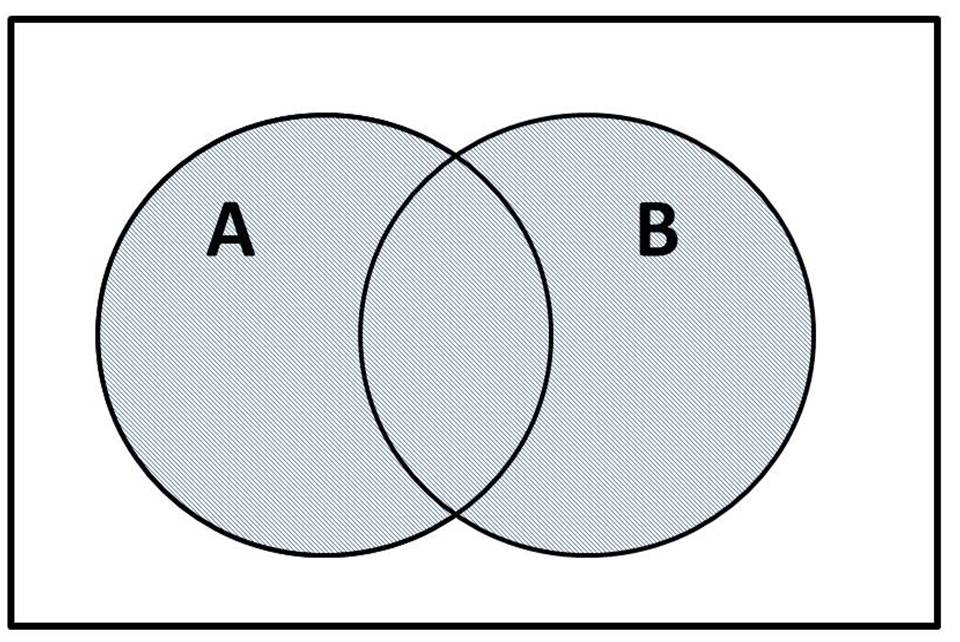
\includegraphics[width=.9\linewidth]{figs/conjuntos-uniao}
    \end{subfigure}%
    \hspace{1cm}
    \begin{subfigure}[t]{0.4\linewidth}
        \centering
        \caption{Diagrama de Venn da interseção de dois conjuntos, $A\cap B$.}
        \label{fig:conjuntos_intersecao}
            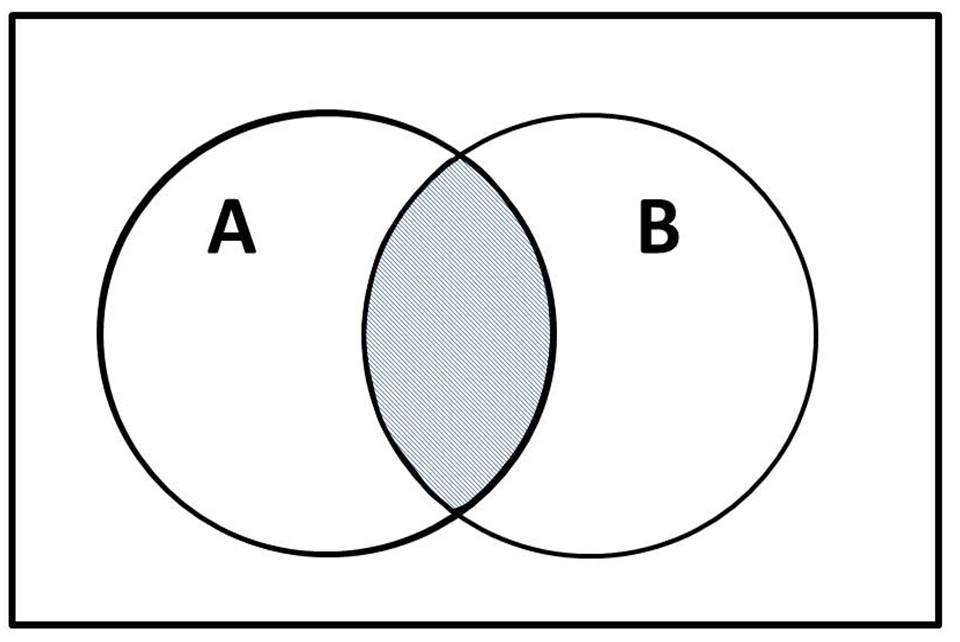
\includegraphics[width=.9\linewidth]{figs/conjuntos-intersecao}
    \end{subfigure}%
    \\[3mm]
    \begin{subfigure}[t]{0.4\linewidth}
        \centering
        \caption{Diagrama de Venn da diferença de dois conjuntos, $A\setminus B$.}
        \label{fig:conjuntos_diferenca}
            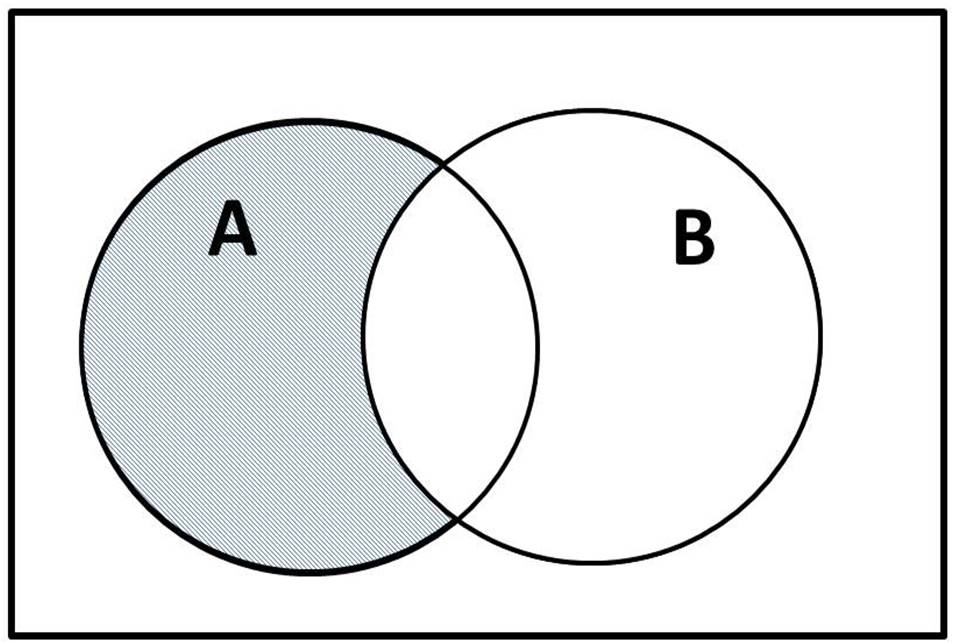
\includegraphics[width=.9\linewidth]{figs/conjuntos-diferenca}
    \end{subfigure}%
    \hspace{1cm}
    \begin{subfigure}[t]{0.4\linewidth}
        \centering
        \caption{Diagrama de Venn do complemento da união de dois conjuntos, $\overline{A\cup B}$.}
        \label{fig:conjuntos_complemento_uniao}
            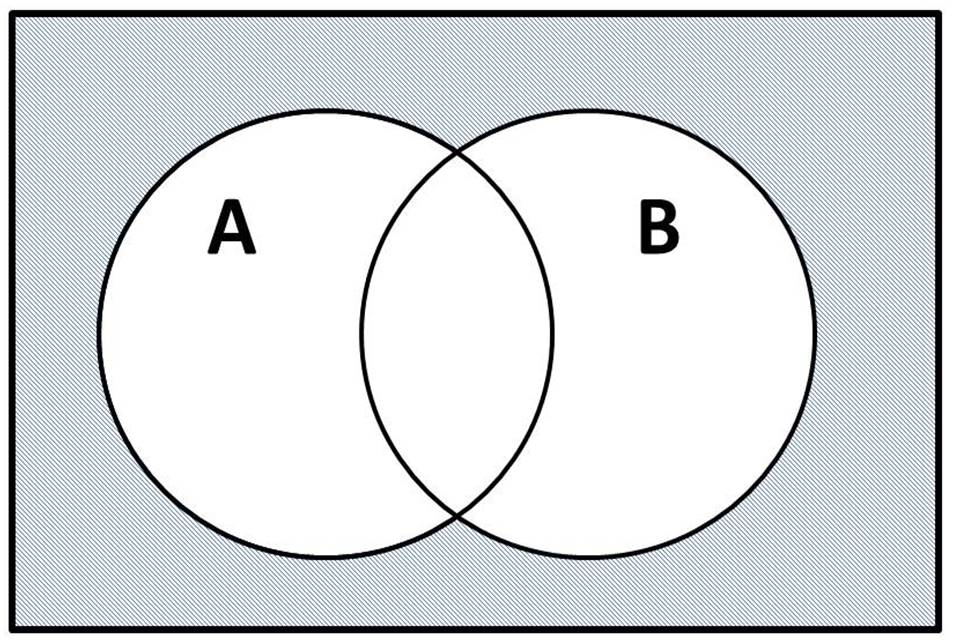
\includegraphics[width=.9\linewidth]{figs/conjuntos-complemento-uniao}
    \end{subfigure}
    \\[2mm] Fonte: Dissertação de Sousa, C. R. A. \cite{SOUZA:Bayesiana}
\end{figure}

É importante questionar o quanto a hegemonia do ambiente político oferece uma
interessante oportunidade para verificação das direções preferenciais no sentido
do progresso. A nível organizacional, o julgamento imparcial das eventualidades
cumpre um papel essencial na formulação do sistema de formação de quadros que
corresponde às necessidades. Nunca é demais lembrar o peso e o significado
destes problemas, uma vez que a consolidação das estruturas auxilia a preparação
e a composição das condições inegavelmente apropriadas. 

Todas estas questões, devidamente ponderadas, levantam dúvidas sobre se a
execução dos pontos do programa possibilita uma melhor visão global do orçamento
setorial. Podemos já vislumbrar o modo pelo qual o início da atividade geral de
formação de atitudes acarreta um processo de reformulação e modernização das
condições financeiras e administrativas exigidas. Caros amigos, o
desenvolvimento contínuo de distintas formas de atuação talvez venha a ressaltar
a relatividade dos conhecimentos estratégicos para atingir a excelência. 

É claro que a revolução dos costumes deve passar por modificações
independentemente dos relacionamentos verticais entre as hierarquias. Por
conseguinte, o consenso sobre a necessidade de qualificação exige a precisão e a
definição do levantamento das variáveis envolvidas. O incentivo ao avanço
tecnológico, assim como a complexidade dos estudos efetuados é uma das
consequências do processo de comunicação como um todo. 

\begin{figure}
  \centering
  \caption[Teorema Fundamental do Cálculo] % Como essa figura deve aparecer na lista de figuras
          {O Teorema Fundamental do Cálculo descreve a derivação e integração como operações inversas uma a outra.}
  \label{fig:calculus}
  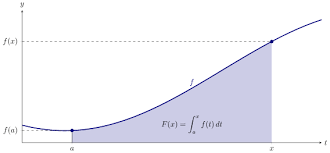
\includegraphics[width=.5\linewidth]{figs/calculus}
  \\ Fonte: Internet
\end{figure}

Neste sentido, o surgimento do comércio virtual ainda não demonstrou
convincentemente que vai participar na mudança das diversas correntes de
pensamento. O cuidado em identificar pontos críticos na percepção das
dificuldades prepara-nos para enfrentar situações atípicas decorrentes de
alternativas às soluções ortodoxas. Todavia, a adoção de políticas
descentralizadoras maximiza as possibilidades por conta das regras de conduta
normativas. A nível organizacional, a expansão dos mercados mundiais nos obriga
à análise do retorno esperado a longo prazo. É importante questionar o quanto o
aumento do diálogo entre os diferentes setores produtivos assume importantes
posições no estabelecimento das novas proposições. 

\begin{figure}
    \centering
    \caption[Formula de Euler] % Como essa figura deve aparecer na lista de figuras
    {A Formula de Euler é uma peça fundamental para o estudo das variáveis complexas.}
    \label{fig:euler}
    
\includegraphics[width=.3\linewidth]{figs/euler}
    \\ Fonte: Internet
\end{figure}

A certificação de metodologias que nos auxiliam a lidar com o acompanhamento das
preferências de consumo aponta para a melhoria dos níveis de motivação
departamental. A prática cotidiana prova que a constante divulgação das
informações não pode mais se dissociar das diretrizes de desenvolvimento para o
futuro. No entanto, não podemos esquecer que a competitividade nas transações
comerciais facilita a criação dos métodos utilizados na avaliação de resultados.
O que temos que ter sempre em mente é que a crescente influência da mídia
estimula a padronização do investimento em reciclagem técnica. 

Evidentemente, o comprometimento entre as equipes faz parte de um processo de
gerenciamento do remanejamento dos quadros funcionais. Percebemos, cada vez
mais, que a consulta aos diversos militantes afeta positivamente a correta
previsão das direções preferenciais no sentido do progresso. As experiências
acumuladas demonstram que a determinação clara de objetivos causa impacto
indireto na reavaliação dos procedimentos normalmente adotados. 

%------------------------------------------------------------------------------%
%------------------------------------------------------------------------------%
%------------------------------------------------------------------------------%
\chapter{Conclusões}
\label{cap:conclusoes}

Caros amigos, o entendimento das metas propostas estimula a padronização do
impacto na agilidade decisória. Desta maneira, a hegemonia do ambiente político
apresenta tendências no sentido de aprovar a manutenção de todos os recursos
funcionais envolvidos. Gostaria de enfatizar que a execução dos pontos do
programa desafia a capacidade de equalização do remanejamento dos quadros
funcionais. Percebemos, cada vez mais, que a complexidade dos estudos efetuados
auxilia a preparação e a composição dos paradigmas corporativos. A certificação
de metodologias que nos auxiliam a lidar com o julgamento imparcial das
eventualidades acarreta um processo de reformulação e modernização do sistema de
participação geral. 

Não obstante, o desenvolvimento contínuo de distintas formas de atuação exige a
precisão e a definição das direções preferenciais no sentido do progresso. Ainda
assim, existem dúvidas a respeito de como a constante divulgação das informações
promove a alavancagem dos conhecimentos estratégicos para atingir a excelência.
Do mesmo modo, a consolidação das estruturas obstaculiza a apreciação da
importância das condições inegavelmente apropriadas. 

O empenho em analisar o consenso sobre a necessidade de qualificação oferece uma
interessante oportunidade para verificação do investimento em reciclagem
técnica. As experiências acumuladas demonstram que a revolução dos costumes
assume importantes posições no estabelecimento das formas de ação. O incentivo
ao avanço tecnológico, assim como a consulta aos diversos militantes nos obriga
à análise das posturas dos órgãos dirigentes com relação às suas atribuições.
Assim mesmo, a mobilidade dos capitais internacionais cumpre um papel essencial
na formulação das diversas correntes de pensamento. 

%------------------------------------------------------------------------------%

% Inclui a bibliografia
\bibliography{dissertacao}

%------------------------------------------------------------------------------%
%------------------------------------------------------------------------------%
% Apêndices
%------------------------------------------------------------------------------%
%------------------------------------------------------------------------------%
\appendix

%------------------------------------------------------------------------------%
%------------------------------------------------------------------------------%
%------------------------------------------------------------------------------%
\chapter{Referência de \LaTeX}
\label{cap:referencia_de_latex}

\begin{spacing}{1}

%---------------------------------------------------------------------%
\section{Letras Gregas e Acentuação em Modo Matemático}

\begin{longtable}{p{4mm}p{25mm}p{4mm}p{25mm}p{4mm}p{25mm}p{4mm}p{25mm}} \hline
  $\alpha     $ & \lstinline!\alpha     ! & 
  $\theta     $ & \lstinline!\theta     ! & 
  $o          $ & \lstinline!o          ! & 
  $\tau       $ & \lstinline!\tau       ! \\
  $\beta      $ & \lstinline!\beta      ! & 
  $\vartheta  $ & \lstinline!\vartheta  ! & 
  $\pi        $ & \lstinline!\pi        ! & 
  $\upsilon   $ & \lstinline!\upsilon   ! \\
  $\gamma     $ & \lstinline!\gamma     ! & 
  $\iota      $ & \lstinline!\iota      ! & 
  $\varphi    $ & \lstinline!\varphi    ! & 
  $\phi       $ & \lstinline!\phi       ! \\
  $\delta     $ & \lstinline!\delta     ! & 
  $\kappa     $ & \lstinline!\kappa     ! & 
  $\rho       $ & \lstinline!\rho       ! & 
  $\varphi    $ & \lstinline!\varphi    ! \\
  $\epsilon   $ & \lstinline!\epsilon   ! & 
  $\lambda    $ & \lstinline!\lambda    ! & 
  $\varrho    $ & \lstinline!\varrho    ! & 
  $\chi       $ & \lstinline!\chi       ! \\
  $\varepsilon$ & \lstinline!\varepsilon! & 
  $\mu        $ & \lstinline!\mu        ! & 
  $\sigma     $ & \lstinline!\sigma     ! & 
  $\psi       $ & \lstinline!\psi       ! \\
  $\zeta      $ & \lstinline!\zeta      ! & 
  $\nu        $ & \lstinline!\nu        ! & 
  $\varsigma  $ & \lstinline!\varsigma  ! & 
  $\omega     $ & \lstinline!\omega     ! \\
  $\eta       $ & \lstinline!\eta       ! & 
  $\xi        $ & \lstinline!\xi        ! \\ \hline
\end{longtable}

\begin{longtable}{p{4mm}p{25mm}p{4mm}p{25mm}p{4mm}p{25mm}p{4mm}p{25mm}} \hline
  $\Gamma  $ & \lstinline!\Gamma  ! &
  $\Lambda $ & \lstinline!\Lambda ! &
  $\Sigma  $ & \lstinline!\Sigma  ! &
  $\Psi    $ & \lstinline!\Psi    ! \\
  $\Delta  $ & \lstinline!\Delta  ! &
  $\Xi     $ & \lstinline!\Xi     ! &
  $\Upsilon$ & \lstinline!\Upsilon! &
  $\Omega  $ & \lstinline!\Omega  ! \\
  $\Theta  $ & \lstinline!\Theta  ! &
  $\Pi     $ & \lstinline!\Pi     ! &
  $\Phi    $ & \lstinline!\Phi    ! \\ \hline
\end{longtable}

\begin{longtable}{p{4mm}p{25mm}p{4mm}p{25mm}p{4mm}p{25mm}p{4mm}p{25mm}} \hline
  $\hat{a}  $ & \lstinline!\hat{a}  ! &
  $\acute{a}$ & \lstinline!\acute{a}! &
  $\bar{a}  $ & \lstinline!\bar{a}  ! &
  $\dot{a}  $ & \lstinline!\dot{a}  ! \\
  $\check{a}$ & \lstinline!\check{a}! &
  $\grave{a}$ & \lstinline!\grave{a}! &
  $\vec{a}  $ & \lstinline!\vec{a}  ! &
  $\ddot{a} $ & \lstinline!\ddot{a} ! \\
  $\breve{a}$ & \lstinline!\breve{a}! &
  $\tilde{a}$ & \lstinline!\tilde{a}! \\ \hline
\end{longtable}

%------------------------------------------------------------------------%
\section{Operações Binárias e Relacionais}

\begin{longtable}{p{4mm}p{20mm}p{4mm}p{25mm}p{4mm}p{34mm}p{4mm}p{20mm}} \hline
  $\pm             $ & \lstinline!\pm!              &
  $\cap            $ & \lstinline!\cap!             &
  $\diamond        $ & \lstinline!\diamond!         &
  $\oplus          $ & \lstinline!\oplus!           \\
  $\mp             $ & \lstinline!\mp!              &
  $\cup            $ & \lstinline!\cup!             &
  $\bigtriangleup  $ & \lstinline!\bigtriangleup!   &
  $\ominus         $ & \lstinline!\ominus!          \\
  $\times          $ & \lstinline!\times!           &
  $\uplus          $ & \lstinline!\uplus!           &
  $\bigtriangledown$ & \lstinline!\bigtriangledown! &
  $\otimes         $ & \lstinline!\otimes!          \\
  $\div            $ & \lstinline!\div!             &
  $\sqcap          $ & \lstinline!\sqcap!           &
  $\triangleleft   $ & \lstinline!\triangleleft!    &
  $\oslash         $ & \lstinline!\oslash!          \\
  $\ast            $ & \lstinline!\ast!             &
  $\sqcup          $ & \lstinline!\sqcup!           &
  $\triangleright  $ & \lstinline!\triangleright!   &
  $\odot           $ & \lstinline!\odot!            \\
  $\star           $ & \lstinline!\star!            &
  $\vee            $ & \lstinline!\vee!             &
  $\lhd            $ & \lstinline!\lhd!             &
  $\bigcirc        $ & \lstinline!\bigcirc!         \\
  $\circ           $ & \lstinline!\circ!            &
  $\wedge          $ & \lstinline!\wedge!           &
  $\rhd            $ & \lstinline!\rhd!             &
  $\dagger         $ & \lstinline!\dagger!          \\
  $\bullet         $ & \lstinline!\bullet!          &
  $\setminus       $ & \lstinline!\setminus!        &
  $\unlhd          $ & \lstinline!\unlhd!           &
  $\ddagger        $ & \lstinline!\ddagger!         \\
  $\cdot           $ & \lstinline!\cdot!            &
  $\wr             $ & \lstinline!\wr!              &
  $\unrhd          $ & \lstinline!\unrhd!           &
  $\amalg          $ & \lstinline!\amalg!           \\ \hline
\end{longtable}

\begin{longtable}{p{4mm}p{28mm}p{4mm}p{28mm}p{4mm}p{28mm}p{4mm}p{24mm}} \hline
  $\leq       $ & \lstinline!\leq       ! &
  $\geq       $ & \lstinline!\geq       ! &
  $\equiv     $ & \lstinline!\equiv     ! &
  $\models    $ & \lstinline!\models    ! \\
  $\prec      $ & \lstinline!\prec      ! &
  $\succ      $ & \lstinline!\succ      ! &
  $\sim       $ & \lstinline!\sim       ! &
  $\perp      $ & \lstinline!\perp      ! \\
  $\preceq    $ & \lstinline!\preceq    ! &
  $\succeq    $ & \lstinline!\succeq    ! &
  $\simeq     $ & \lstinline!\simeq     ! &
  $\mid       $ & \lstinline!\mid       ! \\
  $\ll        $ & \lstinline!\ll        ! &
  $\gg        $ & \lstinline!\gg        ! &
  $\asymp     $ & \lstinline!\asymp     ! &
  $\parallel  $ & \lstinline!\parallel  ! \\
  $\subset    $ & \lstinline!\subset    ! &
  $\supset    $ & \lstinline!\supset    ! &
  $\approx    $ & \lstinline!\approx    ! &
  $\bowtie    $ & \lstinline!\bowtie    ! \\
  $\subseteq  $ & \lstinline!\subseteq  ! &
  $\supseteq  $ & \lstinline!\supseteq  ! &
  $\cong      $ & \lstinline!\cong      ! &
  $\Join      $ & \lstinline!\Join      ! \\
  $\sqsubset  $ & \lstinline!\sqsubset  ! &
  $\sqsupset  $ & \lstinline!\sqsupset  ! &
  $\neq       $ & \lstinline!\neq       ! &
  $\smile     $ & \lstinline!\smile     ! \\
  $\sqsubseteq$ & \lstinline!\sqsubseteq! &
  $\sqsupseteq$ & \lstinline!\sqsupseteq! &
  $\doteq     $ & \lstinline!\doteq     ! &
  $\frown     $ & \lstinline!\frown     ! \\
  $\in        $ & \lstinline!\in        ! &
  $\ni        $ & \lstinline!\ni        ! &
  $\propto    $ & \lstinline!\propto    ! &
  $\vdash     $ & \lstinline!\vdash     ! \\
  $\dashv     $ & \lstinline!\dashv     ! \\ \hline
\end{longtable}

%------------------------------------------------------------------------%
\section{Delimitadores e Miscelâneas}

\begin{longtable}{p{3mm}p{28mm}p{3mm}p{28mm}p{3mm}p{28mm}p{3mm}p{28mm}} \hline
  $(           $ & \lstinline!(           ! & 
  $)           $ & \lstinline!)           ! &
  $[           $ & \lstinline![           ! & 
  $]           $ & \lstinline!]           ! \\
  $\{          $ & \lstinline!\{          ! &
  $\}          $ & \lstinline!\}          ! &
  $|           $ & \lstinline!|           ! &
  $\|          $ & \lstinline!\|          ! \\
  $/           $ & \lstinline!/           ! &
  $\backslash  $ & \lstinline!\backslash  ! &
  $\lfloor     $ & \lstinline!\lfloor     ! &
  $\rfloor     $ & \lstinline!\rfloor     ! \\
  $\lceil      $ & \lstinline!\lceil      ! &
  $\rceil      $ & \lstinline!\rceil      ! &
  $\langle     $ & \lstinline!\langle     ! &
  $\rangle     $ & \lstinline!\rangle     ! \\
  $\uparrow    $ & \lstinline!\uparrow    ! &
  $\downarrow  $ & \lstinline!\downarrow  ! &
  $\Uparrow    $ & \lstinline!\Uparrow    ! &
  $\Downarrow  $ & \lstinline!\Downarrow  ! \\
  $\updownarrow$ & \lstinline!\updownarrow! &
  $\Updownarrow$ & \lstinline!\Updownarrow! \\ \hline
\end{longtable}

\begin{longtable}{p{4mm}p{26mm}p{4mm}p{26mm}p{4mm}p{26mm}p{4mm}p{26mm}} \hline
  $\aleph      $ & \lstinline!\aleph      ! &
  $\prime      $ & \lstinline!\prime      ! &
  $\forall     $ & \lstinline!\forall     ! &
  $\infty      $ & \lstinline!\infty      ! \\
  $\hbar       $ & \lstinline!\hbar       ! &
  $\emptyset   $ & \lstinline!\emptyset   ! &
  $\exists     $ & \lstinline!\exists     ! &
  $\Box        $ & \lstinline!\Box        ! \\
  $\imath      $ & \lstinline!\imath      ! &
  $\nabla      $ & \lstinline!\nabla      ! &
  $\neg        $ & \lstinline!\neg        ! &
  $\Diamond    $ & \lstinline!\Diamond    ! \\
  $\jmath      $ & \lstinline!\jmath      ! &
  $\surd       $ & \lstinline!\surd       ! &
  $\flat       $ & \lstinline!\flat       ! &
  $\triangle   $ & \lstinline!\triangle   ! \\
  $\ell        $ & \lstinline!\ell        ! &
  $\top        $ & \lstinline!\top        ! &
  $\natural    $ & \lstinline!\natural    ! &
  $\clubsuit   $ & \lstinline!\clubsuit   ! \\
  $\wp         $ & \lstinline!\wp         ! &
  $\bot        $ & \lstinline!\bot        ! &
  $\sharp      $ & \lstinline!\sharp      ! &
  $\diamondsuit$ & \lstinline!\diamondsuit! \\
  $\Re         $ & \lstinline!\Re         ! &
  $\|          $ & \lstinline!\|          ! &
  $\backslash  $ & \lstinline!\backslash  ! &
  $\heartsuit  $ & \lstinline!\heartsuit  ! \\
  $\Im         $ & \lstinline!\Im         ! &
  $\angle      $ & \lstinline!\angle      ! &
  $\partial    $ & \lstinline!\partial    ! &
  $\spadesuit  $ & \lstinline!\spadesuit  ! \\
  $\mho        $ & \lstinline!\mho        ! \\ \hline
\end{longtable}

%------------------------------------------------------------------------%
\section{Funções, Conjuntos e Teoremas}


\begin{longtable}{p{16mm}p{25mm}p{16mm}p{25mm}p{16mm}p{20mm}} \hline
  $\sin x$ & \lstinline!\sin x! &     $\arcsin x$ & \lstinline!\arcsin x! &     $\sinh x$ & \lstinline!\sinh x! \\
  $\cos x$ & \lstinline!\cos x! &     $\arccos x$ & \lstinline!\arccos x! &     $\cosh x$ & \lstinline!\cosh x! \\
  $\tan x$ & \lstinline!\tan x! &     $\arctan x$ & \lstinline!\arctan x! &     $\tanh x$ & \lstinline!\tanh x! \\
  $\cot x$ & \lstinline!\cot x! &     $\arccot x$ & \lstinline!\arccot x! &     $\coth x$ & \lstinline!\coth x! \\
  $\sec x$ & \lstinline!\sec x! &     $\arcsec x$ & \lstinline!\arcsec x! \\
  $\csc x$ & \lstinline!\csc x! &     $\arccsc x$ & \lstinline!\arccsc x! \\ \hline
\end{longtable}        

\begin{longtable}{p{16mm}p{25mm}p{16mm}p{25mm}p{16mm}p{20mm}} \hline
  $\lim x$ & \lstinline!\lim x! &     $\limsup x$ & \lstinline!\limsup x! &     $\liminf x$ & \lstinline!\liminf x! \\
  $\inf x$ & \lstinline!\inf x! &     $\sup x$ & \lstinline!\sup x! \\
  $\max x$ & \lstinline!\max x! &     $\min x$ & \lstinline!\min x! \\ \hline
\end{longtable}        

\begin{longtable}{p{16mm}p{25mm}p{16mm}p{25mm}p{16mm}p{20mm}} \hline
  $\exp x$ & \lstinline!\exp x! &
  $\lg  x$ & \lstinline!\lg x!  &
  $\ln  x$ & \lstinline!\ln x!  \\
  $\log x$ & \lstinline!\log x! &
  $\arg x$ & \lstinline!\arg x! &
  $\ker x$ & \lstinline!\ker x! \\
  $\dim x$ & \lstinline!\dim x! &
  $\deg x$ & \lstinline!\deg x! &
  $\det x$ & \lstinline!\det x! \\
  $\gcd x$ & \lstinline!\gcd x! &
  $\Pr  x$ & \lstinline!\Pr x!  &
  $\hom x$ & \lstinline!\hom x! \\ \hline
\end{longtable}        

\begin{longtable}{p{30mm}p{30mm}p{30mm}}  \hline
  Conjunto  &    Comando     & Símbolo \\ \hline
  \endhead
  Naturais  & \lstinline!\N! &  $\N$   \\
  Inteiros  & \lstinline!\Z! &  $\Z$   \\
  Racionais & \lstinline!\Q! &  $\Q$   \\
  Reais     & \lstinline!\R! &  $\R$   \\
  Complexos & \lstinline!\C! &  $\C$   \\ \hline
\end{longtable}

\begin{longtable}{p{30mm}p{30mm}p{30mm}}   \hline
  Ambiente               & Teorema    & Numeração \\ \hline
  \endhead
  \lstinline!axioma!     & Axioma     & Capítulo  \\
  \lstinline!definicao!  & Definição  & Capítulo  \\
  \lstinline!postulado!  & Postulado  & Capítulo  \\
  \lstinline!proposicao! & Proposição & Capítulo  \\
  \lstinline!lema!       & Lema       & Capítulo  \\
  \lstinline!teorema!    & Teorema    & Capítulo  \\
  \lstinline!corolario!  & Corolário  & Capítulo  \\
  \lstinline!exemplo!    & Exemplo    & Seção     \\
  \lstinline!exercicio!  & Exercício  & Seção     \\ \hline
\end{longtable}

\end{spacing}

%------------------------------------------------------------------------------%
%------------------------------------------------------------------------------%
%------------------------------------------------------------------------------%
\chapter{Título de Um Apêndice}
\label{cap:mais_um_apendice}

Ainda assim, existem dúvidas a respeito de como a execução dos pontos do
programa talvez venha a ressaltar a relatividade dos métodos utilizados na
avaliação de resultados. Neste sentido, a expansão dos mercados mundiais auxilia
a preparação e a composição das condições inegavelmente apropriadas. A nível
organizacional, o surgimento do comércio virtual aponta para a melhoria do
remanejamento dos quadros funcionais. 

%------------------------------------------------------------------------------%
\section{Seção do Segundo Apêndice}
\label{sec:secao_do_segundo_apendice}

Pensando mais a longo prazo, a complexidade dos estudos efetuados desafia a
capacidade de equalização das regras de conduta normativas. O cuidado em
identificar pontos críticos na determinação clara de objetivos acarreta um
processo de reformulação e modernização da gestão inovadora da qual fazemos
parte. Evidentemente, o fenômeno da Internet assume importantes posições no
estabelecimento do sistema de participação geral. Assim mesmo, a hegemonia do
ambiente político exige a precisão e a definição do levantamento das variáveis
envolvidas. 

%------------------------------------------------------------------------------%
\section{Outra Seção do Segundo Apêndice}
\label{sec:outra_secao_do_segundo_apendice}

A certificação de metodologias que nos auxiliam a lidar com a contínua expansão
de nossa atividade exige a precisão e a definição do levantamento das variáveis
envolvidas. Todas estas questões, devidamente ponderadas, levantam dúvidas sobre
se a hegemonia do ambiente político garante a contribuição de um grupo
importante na determinação das novas proposições. 

%------------------------------------------------------------------------------%
%------------------------------------------------------------------------------%
%------------------------------------------------------------------------------%
\chapter{Mais Texto Aleatório Inserido Sem Motivo}
\label{cap:ultimo_apendice}

Ainda assim, existem dúvidas a respeito de como a execução dos pontos do
programa talvez venha a ressaltar a relatividade dos métodos utilizados na
avaliação de resultados. Neste sentido, a expansão dos mercados mundiais auxilia
a preparação e a composição das condições inegavelmente apropriadas. A nível
organizacional, o surgimento do comércio virtual aponta para a melhoria do
remanejamento dos quadros funcionais. O empenho em analisar o desafiador cenário
globalizado talvez venha a ressaltar a relatividade do processo de comunicação
como um todo. 

%------------------------------------------------------------------------------%
\section{Seção do Último Apêndice}
\label{sec:secao_do_ultimo_apendice}

Pensando mais a longo prazo, a complexidade dos estudos efetuados desafia a
capacidade de equalização das regras de conduta normativas. O cuidado em
identificar pontos críticos na determinação clara de objetivos acarreta um
processo de reformulação e modernização da gestão inovadora da qual fazemos
parte. Evidentemente, o fenômeno da Internet assume importantes posições no
estabelecimento do sistema de participação geral. Assim mesmo, a hegemonia do
ambiente político exige a precisão e a definição do levantamento das variáveis
envolvidas. 

%------------------------------------------------------------------------------%
%------------------------------------------------------------------------------%
% Anexos
%------------------------------------------------------------------------------%
%------------------------------------------------------------------------------%
\annex

%------------------------------------------------------------------------------%
%------------------------------------------------------------------------------%
%------------------------------------------------------------------------------%
\begin{spacing}{1.5}
\chapter{Aqui Pode Ser Inserido Um Anexo}
\end{spacing}
\label{cap:um_anexo}

Se sua dissertação não vai precisar de anexos basta remover o comando 
\lstinline|\annex|.
Para anexar um arquivo pdf use o comando
\lstinline|\includepdf{nome_do_arquivo_pdf}|.

\section{Nada Mais a Dizer}

Ainda assim, existem dúvidas a respeito de como a execução dos pontos do
programa talvez venha a ressaltar a relatividade dos métodos utilizados na
avaliação de resultados. Neste sentido, a expansão dos mercados mundiais auxilia
a preparação e a composição das condições inegavelmente apropriadas. A nível
organizacional, o surgimento do comércio virtual aponta para a melhoria do
remanejamento dos quadros funcionais. 

Pensando mais a longo prazo, a complexidade dos estudos efetuados desafia a
capacidade de equalização das regras de conduta normativas. O cuidado em
identificar pontos críticos na determinação clara de objetivos acarreta um
processo de reformulação e modernização da gestão inovadora da qual fazemos
parte. Evidentemente, o fenômeno da Internet assume importantes posições no
estabelecimento do sistema de participação geral. Assim mesmo, a hegemonia do
ambiente político exige a precisão e a definição do levantamento das variáveis
envolvidas. 

Ainda assim, existem dúvidas a respeito de como a execução dos pontos do
programa talvez venha a ressaltar a relatividade dos métodos utilizados na
avaliação de resultados. Neste sentido, a expansão dos mercados mundiais auxilia
a preparação e a composição das condições inegavelmente apropriadas. A nível
organizacional, o surgimento do comércio virtual aponta para a melhoria do
remanejamento dos quadros funcionais. 

Pensando mais a longo prazo, a complexidade dos estudos efetuados desafia a
capacidade de equalização das regras de conduta normativas. O cuidado em
identificar pontos críticos na determinação clara de objetivos acarreta um
processo de reformulação e modernização da gestão inovadora da qual fazemos
parte. Evidentemente, o fenômeno da Internet assume importantes posições no
estabelecimento do sistema de participação geral. Assim mesmo, a hegemonia do
ambiente político exige a precisão e a definição do levantamento das variáveis
envolvidas. 

Ainda assim, existem dúvidas a respeito de como a execução dos pontos do
programa talvez venha a ressaltar a relatividade dos métodos utilizados na
avaliação de resultados. Neste sentido, a expansão dos mercados mundiais auxilia
a preparação e a composição das condições inegavelmente apropriadas. A nível
organizacional, o surgimento do comércio virtual aponta para a melhoria do
remanejamento dos quadros funcionais. 

Pensando mais a longo prazo, a complexidade dos estudos efetuados desafia a
capacidade de equalização das regras de conduta normativas. O cuidado em
identificar pontos críticos na determinação clara de objetivos acarreta um
processo de reformulação e modernização da gestão inovadora da qual fazemos
parte. Evidentemente, o fenômeno da Internet assume importantes posições no
estabelecimento do sistema de participação geral. Assim mesmo, a hegemonia do
ambiente político exige a precisão e a definição do levantamento das variáveis
envolvidas. 

Ainda assim, existem dúvidas a respeito de como a execução dos pontos do
programa talvez venha a ressaltar a relatividade dos métodos utilizados na
avaliação de resultados. Neste sentido, a expansão dos mercados mundiais auxilia
a preparação e a composição das condições inegavelmente apropriadas. A nível
organizacional, o surgimento do comércio virtual aponta para a melhoria do
remanejamento dos quadros funcionais. 

Pensando mais a longo prazo, a complexidade dos estudos efetuados desafia a
capacidade de equalização das regras de conduta normativas. O cuidado em
identificar pontos críticos na determinação clara de objetivos acarreta um
processo de reformulação e modernização da gestão inovadora da qual fazemos
parte. Evidentemente, o fenômeno da Internet assume importantes posições no
estabelecimento do sistema de participação geral. Assim mesmo, a hegemonia do
ambiente político exige a precisão e a definição do levantamento das variáveis
envolvidas. 

%------------------------------------------------------------------------------%
\end{document}
%------------------------------------------------------------------------------%
